
\chapter{多個語音離散單元}   \newcommand{\jefftablesep}{\vspace{0.5cm}}
\renewcommand{\arraystretch}{0.7}
\newcommand{\jcm}[1]{}


    {  \jeffcomment{bef analysis} 
{  \jeffcomment{pre}   
\section{動機}              本章嘗試分詞法。
\section{相關研究}   像 Wav2seq \cite{wu_wav2seq_2023}  等是相關研究。
\section{分詞方法}   這邊講述 BPE、Unigram 等演算法具體怎麼實行。}
\section{衡量方式}
  本章節沿用上一章節 LibriSpeech 資料集的 train-clean-100 訓練子集,以及相同的分析數據以進行比對。由於與上一章節的差異僅在分詞方法的引入,因此數據結果將多紀錄分詞前後序列長度的變化;其他操控變因包含分詞方法與詞表大小。考慮到語音訊號本身不如英語等文字,在書寫時就已經具備空格分隔單詞,因此以下分析結果皆採用 SentencePiece 套件中實作之單一詞演算法為分詞方法,並比較詞表大小 500、1000、8000、10000、20000 五種設定的結果差異。(空間不足時則僅呈現 500、1000、10000 三種設定的趨勢。)  }  % 前面的內容

\section{分析結果} 
{
  承繼上一個章節的分析方法,我們先對照純度與機率熱圖兩者的對照,並且以語音學排序呈現,觀察聲學片段與音位之間兩者的分佈關係。

\subsection{由聲學片段角度探討}
{
\subsubsection{聲學片段數量的影響}

{
    {
        \newcommand{\tempwidth}[0]{0.8\linewidth}
        \begin{figure}
             \centering
             \begin{subfigure}{\textwidth}
                 \centering
                 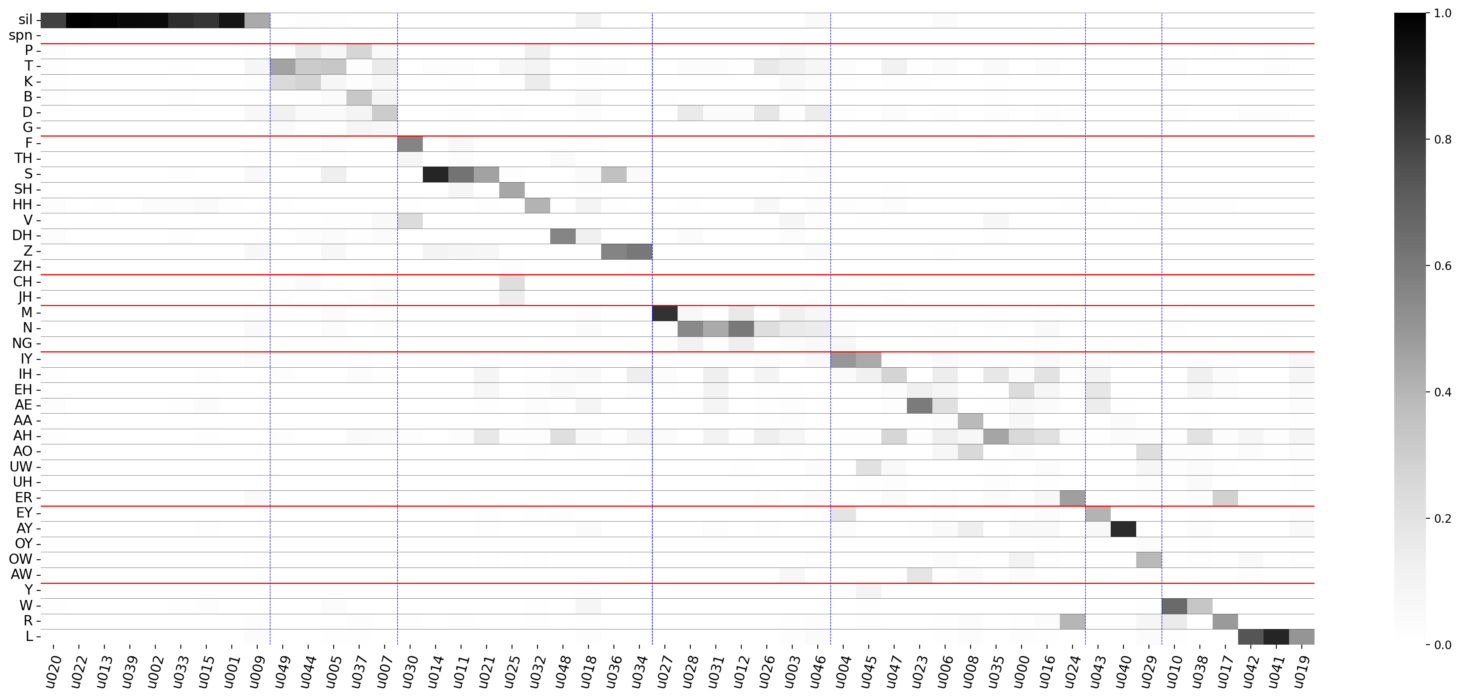
\includegraphics[width=\tempwidth]{feasiblefigs/ch4figs/hub-u050-ap0000-givenunit-byphn.png}
                 \caption{離散單元}
                 \label{fig:hub-u050-ap0000-givenunit-byphn}
             \end{subfigure}
             \vfill
             \begin{subfigure}{\textwidth}
                 \centering
                 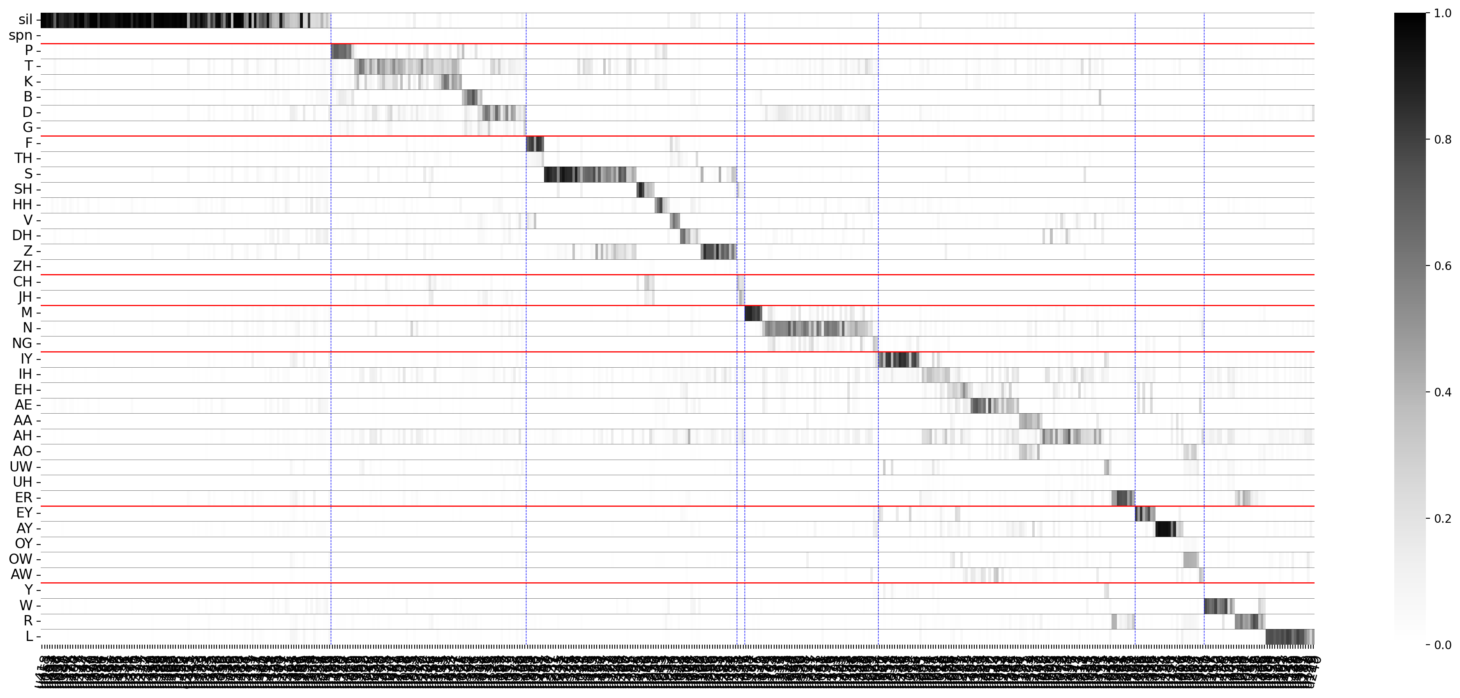
\includegraphics[width=\tempwidth]{feasiblefigs/ch4figs/hub-u050-ap0500-givenunit-byphn.png}
                 \caption{500 種次詞單位}
                 \label{fig:hub-u050-ap0500-givenunit-byphn}
             \end{subfigure}
             \vfill
             \begin{subfigure}{\textwidth}
                 \centering
                 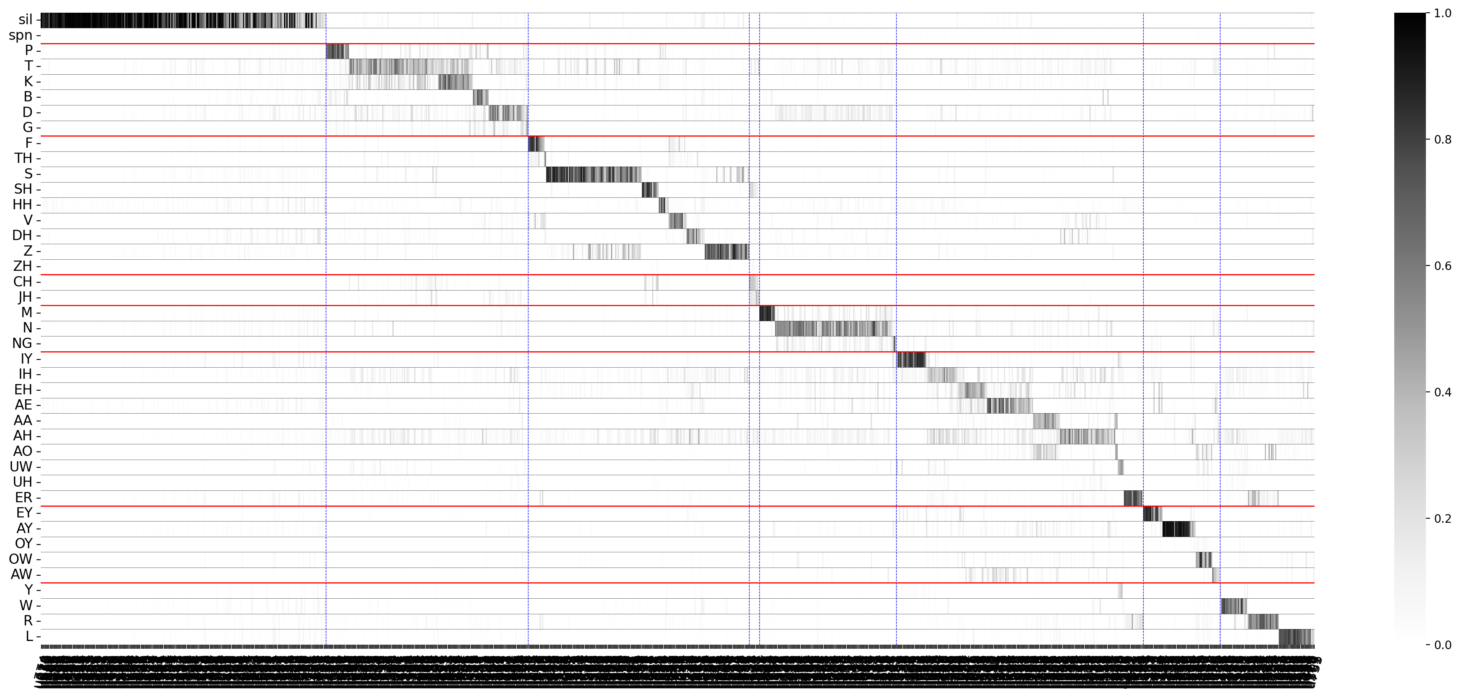
\includegraphics[width=\tempwidth]{feasiblefigs/ch4figs/hub-u050-ap1000-givenunit-byphn.png}
                 \caption{1000 種次詞單位}
                 \label{fig:hub-u050-ap1000-givenunit-byphn}
             \end{subfigure}

             \caption{HuBERT 表徵在 K-平均演算法使用分群數 50 後,}
             比較不同次詞單位數量的條件機率分佈 $p_{y|z}(i | j)$ 熱圖
             \label{fig:hub-u050-comparisons}
        \end{figure}
    }
    {
        \newcommand{\tempwidth}[0]{0.8\linewidth}
        \begin{figure}
             \centering
             \begin{subfigure}{\textwidth}
                 \centering
                 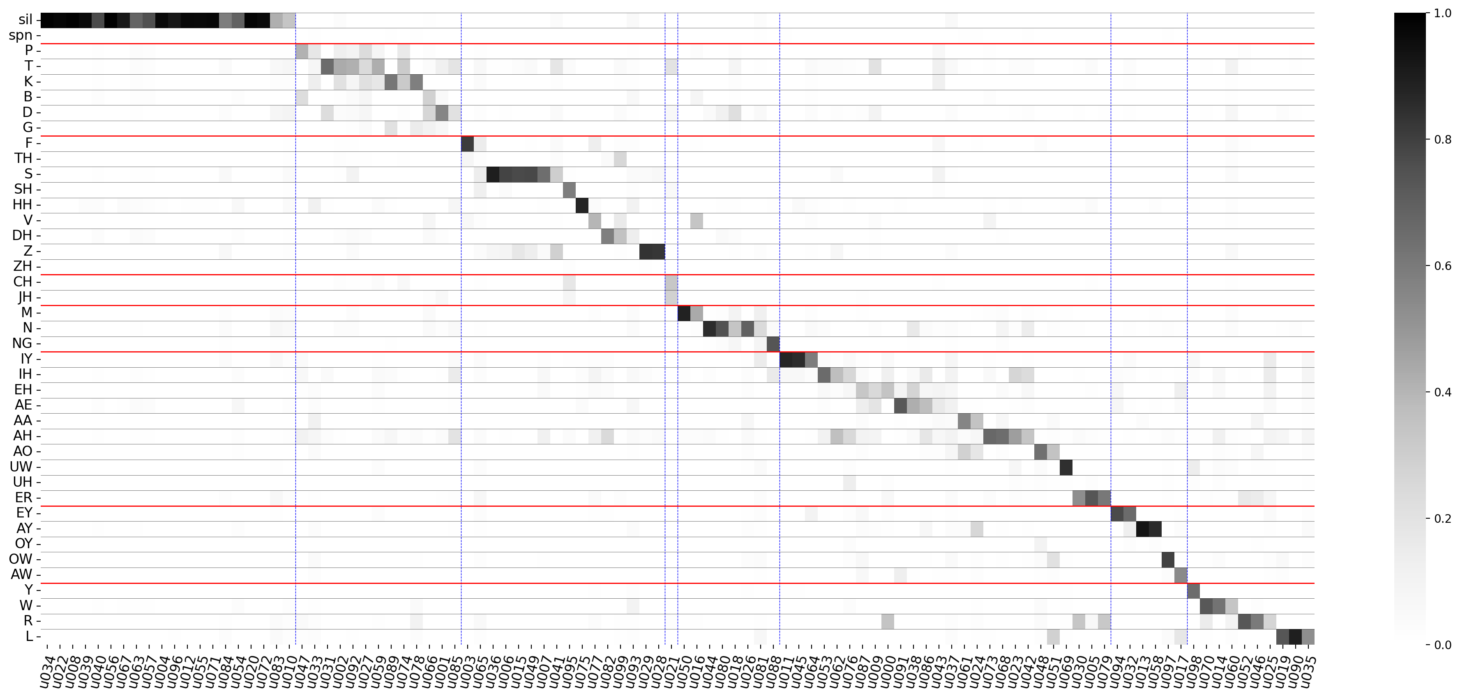
\includegraphics[width=\tempwidth]{feasiblefigs/ch4figs/hub-u100-ap0000-givenunit-byphn.png}
                 \caption{離散單元}
                 \label{fig:hub-u100-ap0000-givenunit-byphn}
             \end{subfigure}
             \vfill
             \begin{subfigure}{\textwidth}
                 \centering
                 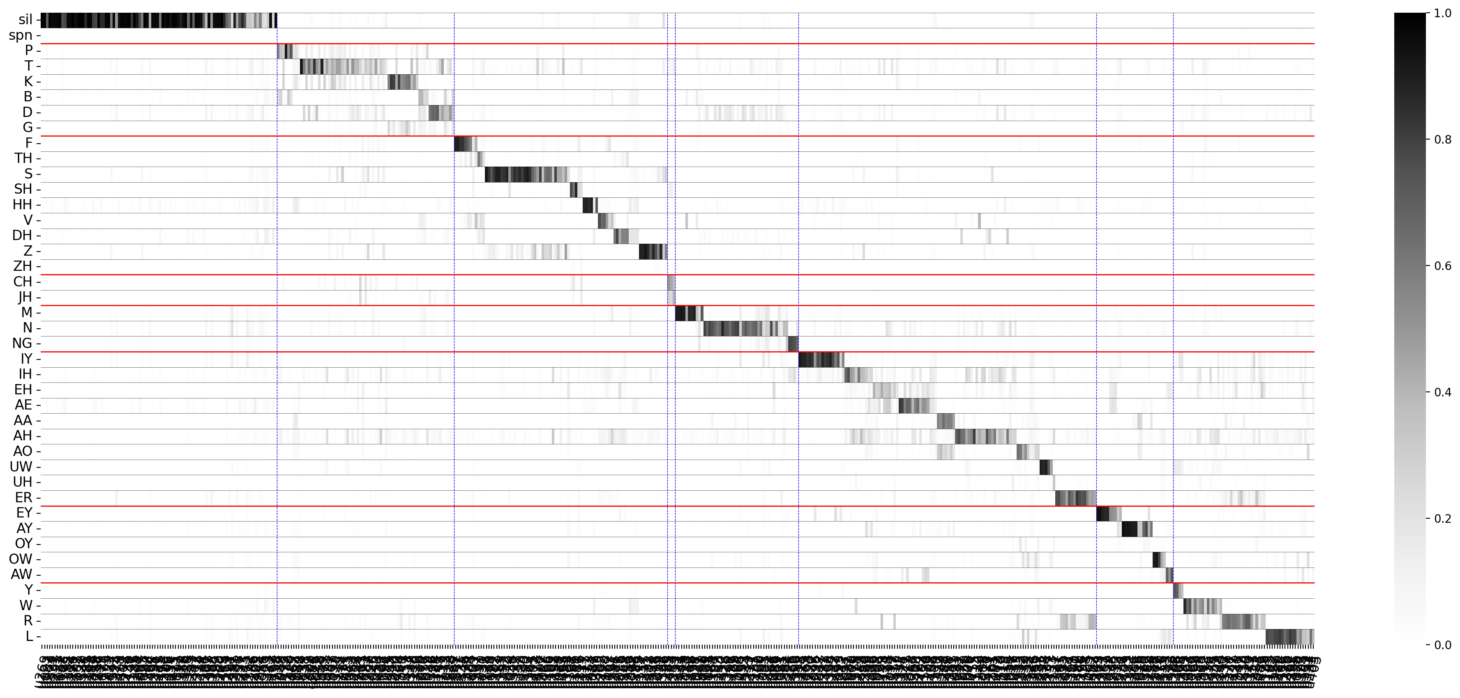
\includegraphics[width=\tempwidth]{feasiblefigs/ch4figs/hub-u100-ap0500-givenunit-byphn.png}
                 \caption{500 種次詞單位}
                 \label{fig:hub-u100-ap0500-givenunit-byphn}
             \end{subfigure}
             \vfill
             \begin{subfigure}{\textwidth}
                 \centering
                 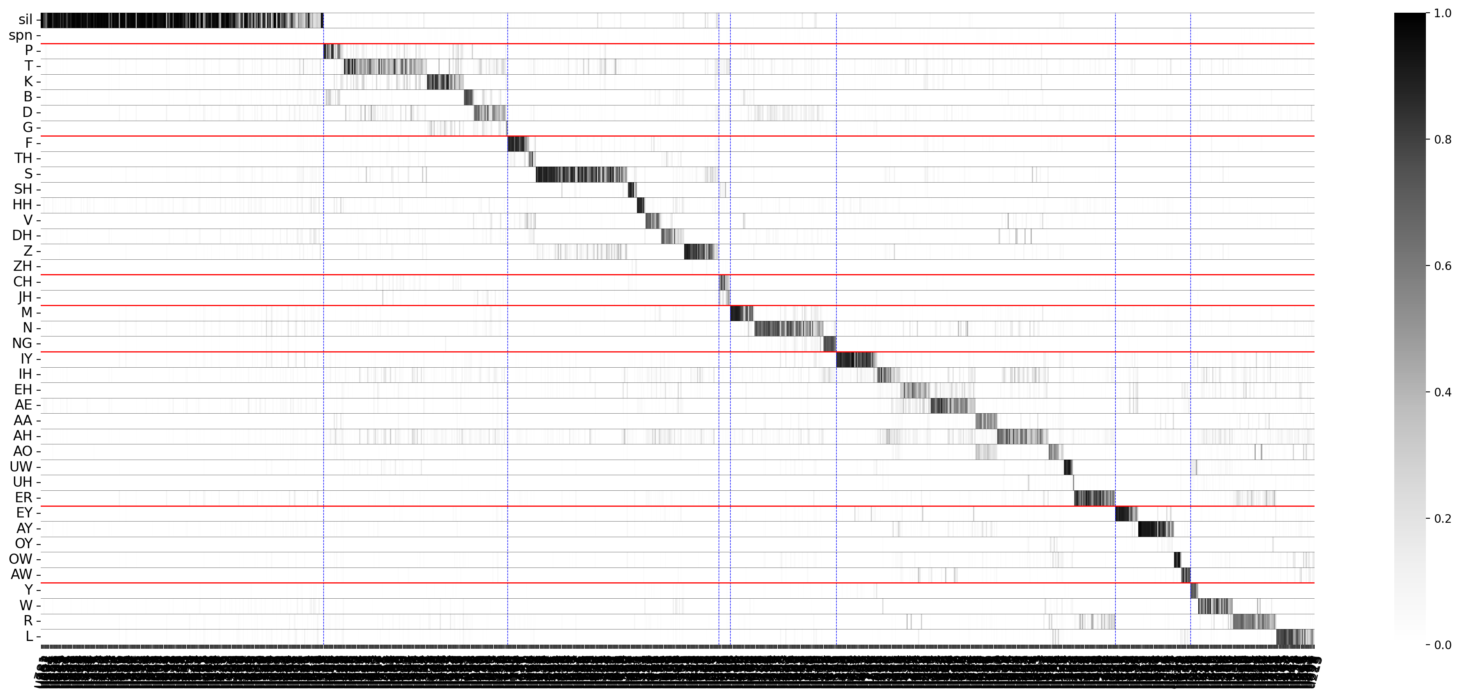
\includegraphics[width=\tempwidth]{feasiblefigs/ch4figs/hub-u100-ap1000-givenunit-byphn.png}
                 \caption{1000 種次詞單位}
                 \label{fig:hub-u100-ap1000-givenunit-byphn}
             \end{subfigure}

             \caption{HuBERT 表徵在 K-平均演算法使用分群數 100 後,}
             比較不同次詞單位數量的條件機率分佈 $p_{y|z}(i | j)$ 熱圖
             \label{fig:hub-u100-comparisons}
        \end{figure}
    }
}

{
    {
        \newcommand{\tempwidth}[0]{0.7\linewidth}
        \begin{figure}
             \centering
             \begin{subfigure}{\textwidth}
                 \centering
                 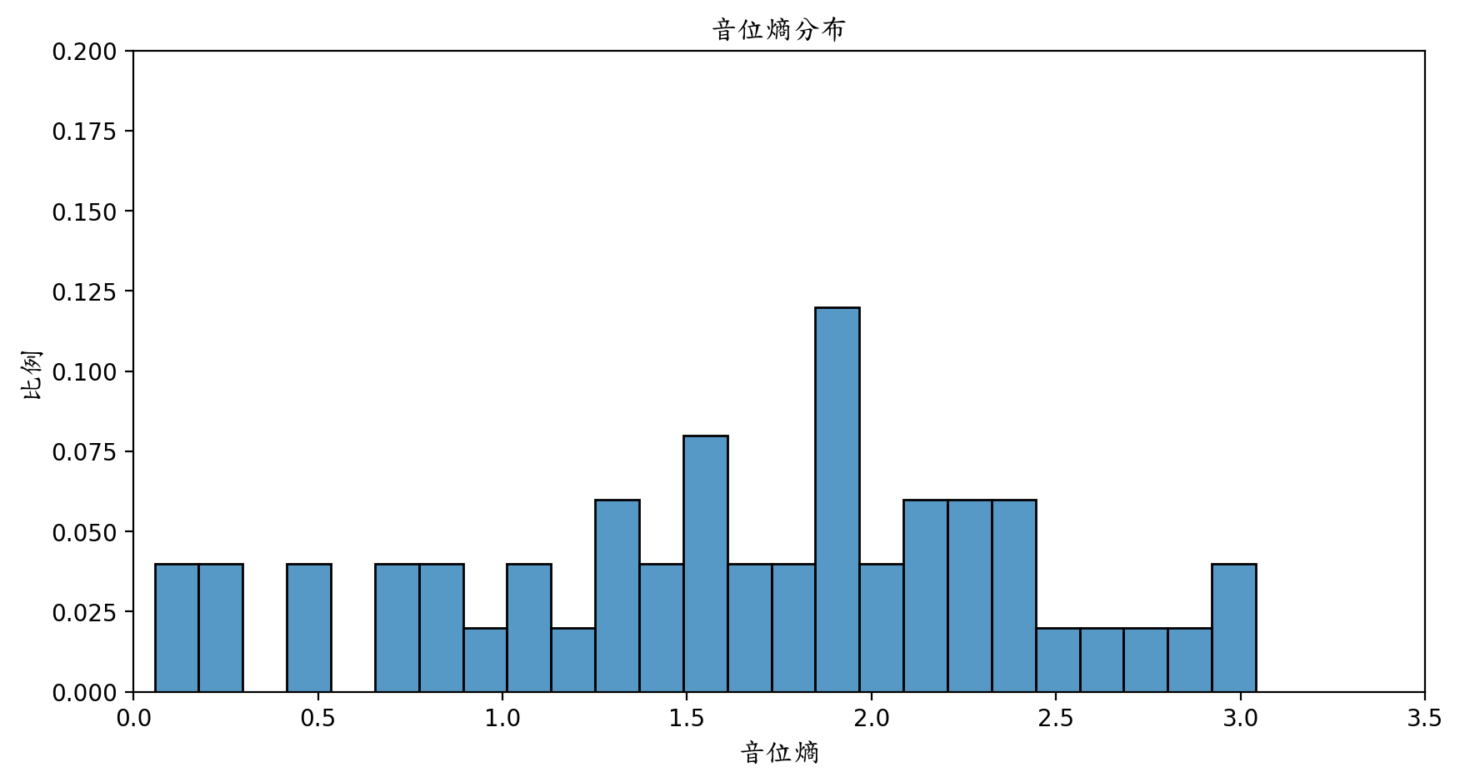
\includegraphics[width=\tempwidth]{feasiblefigs/ch4figs/hub-u050-ap0000-phnent-hist.png}
                 \caption{離散單元}
                 \label{fig:hub-u050-ap0000-phnent-hist}
             \end{subfigure}
             \vfill
             \begin{subfigure}{\textwidth}
                 \centering
                 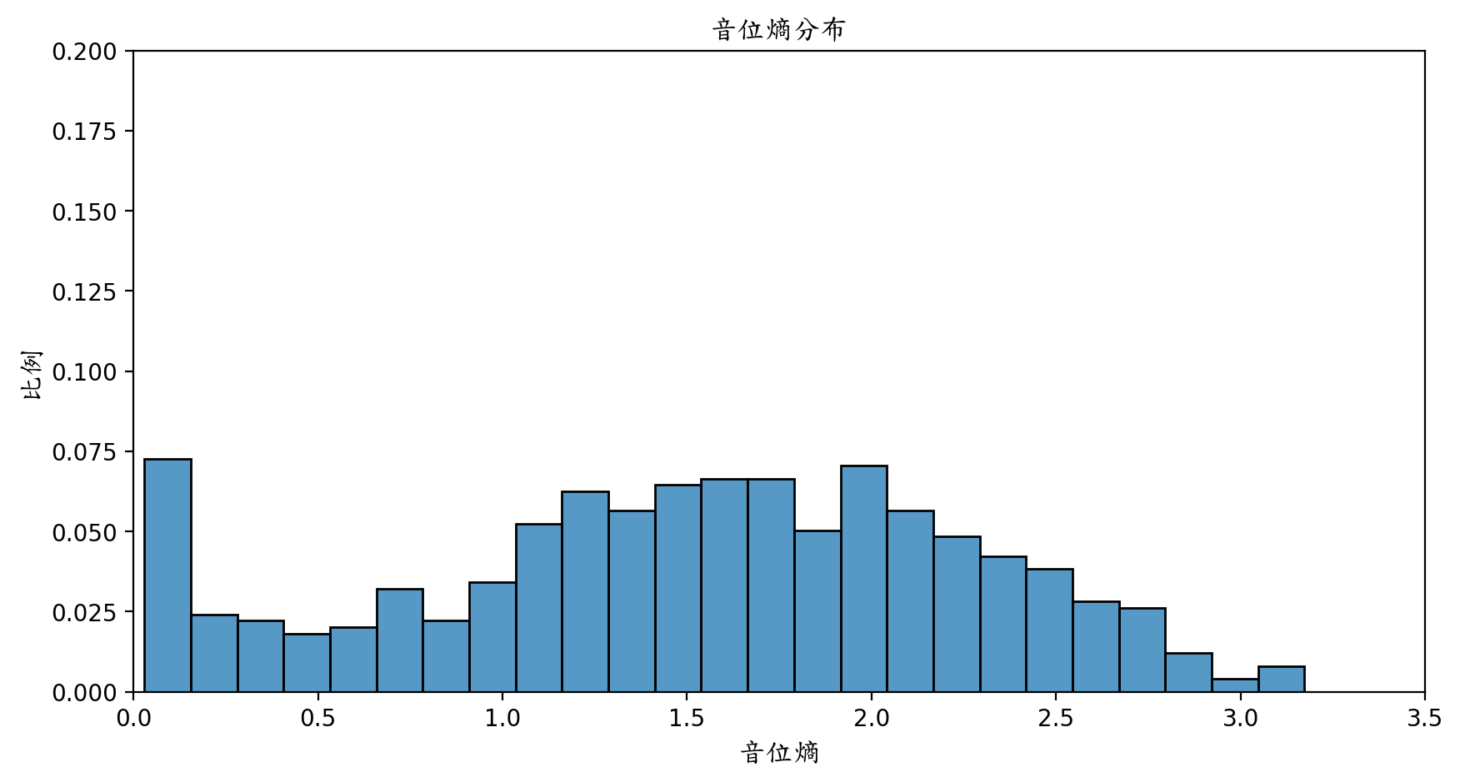
\includegraphics[width=\tempwidth]{feasiblefigs/ch4figs/hub-u050-ap0500-phnent-hist.png}
                 \caption{500 種次詞單位}
                 \label{fig:hub-u050-ap0500-phnent-hist}
             \end{subfigure}
             \vfill
             \begin{subfigure}{\textwidth}
                 \centering
                 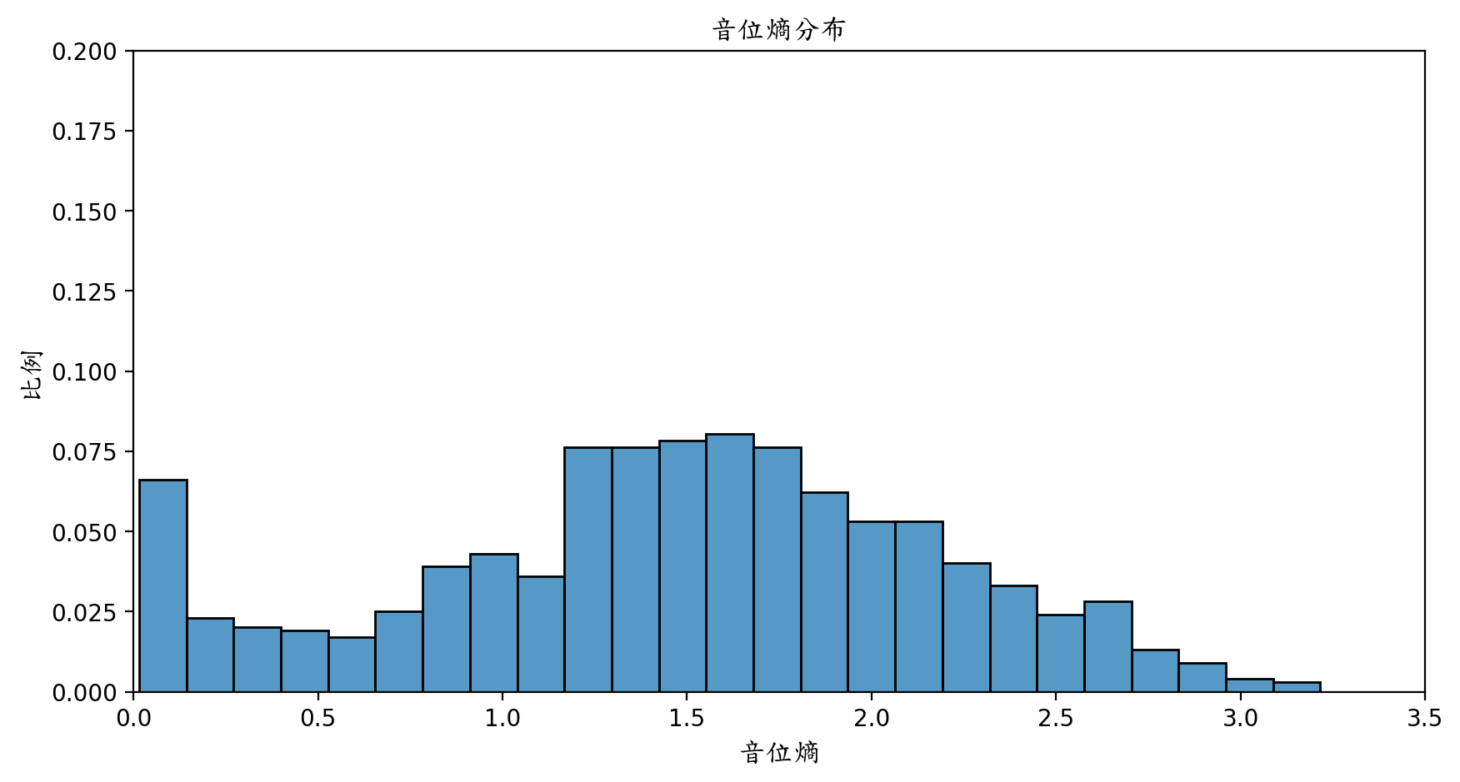
\includegraphics[width=\tempwidth]{feasiblefigs/ch4figs/hub-u050-ap1000-phnent-hist.png}
                 \caption{1000 種次詞單位}
                 \label{fig:hub-u050-ap1000-phnent-hist}
             \end{subfigure}

             \caption{HuBERT 表徵在 K-平均演算法使用分群數 50 後,}
             比較不同次詞單位數量的條音位條件熵 $H(y|z)$ 直方圖
             \label{fig:hub-u050-hist-comparisons}
        \end{figure}
    }
    {
        \newcommand{\tempwidth}[0]{0.7\linewidth}
        \begin{figure}
             \centering
             \begin{subfigure}{\textwidth}
                 \centering
                 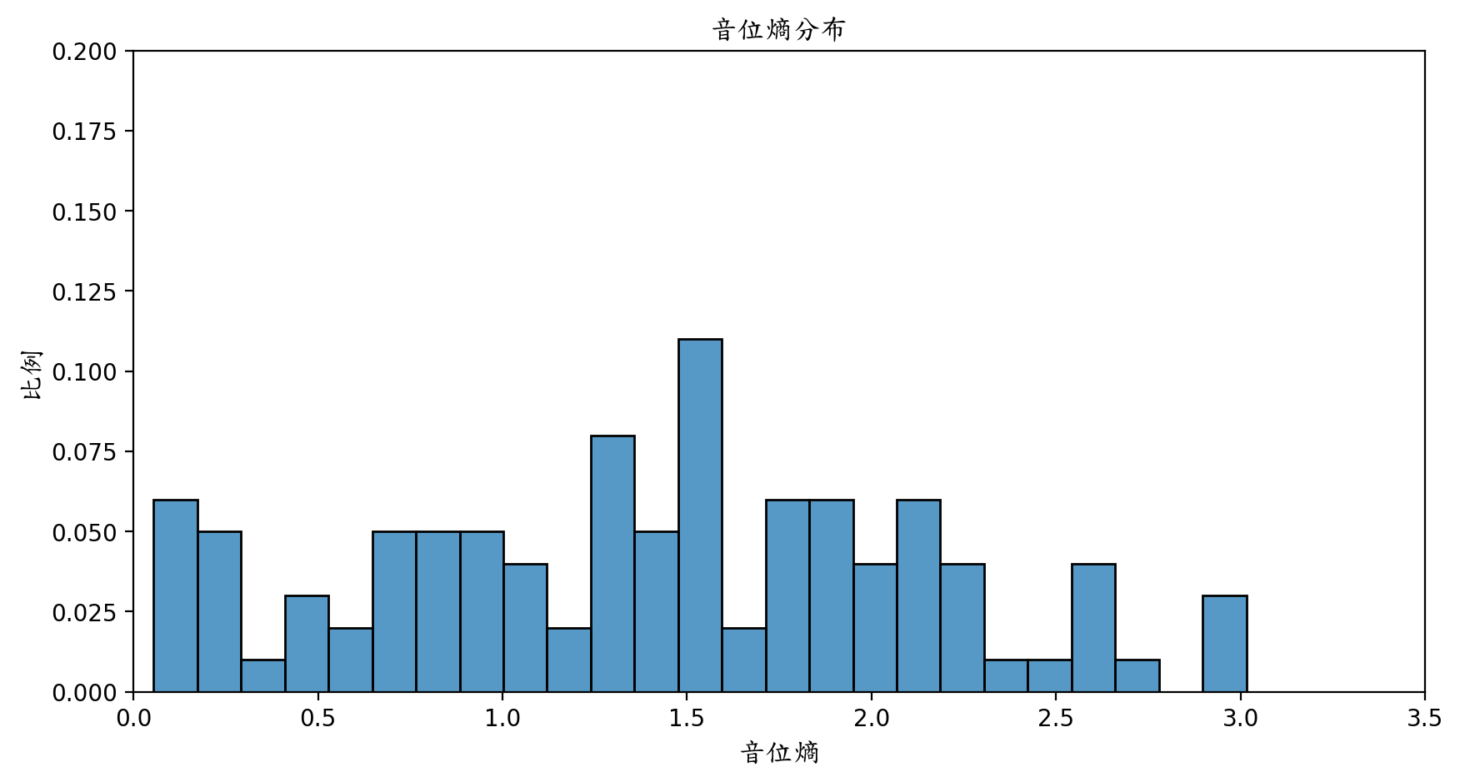
\includegraphics[width=\tempwidth]{feasiblefigs/ch4figs/hub-u100-ap0000-phnent-hist.png}
                 \caption{離散單元}
                 \label{fig:hub-u100-ap0000-phnent-hist}
             \end{subfigure}
             \vfill
             \begin{subfigure}{\textwidth}
                 \centering
                 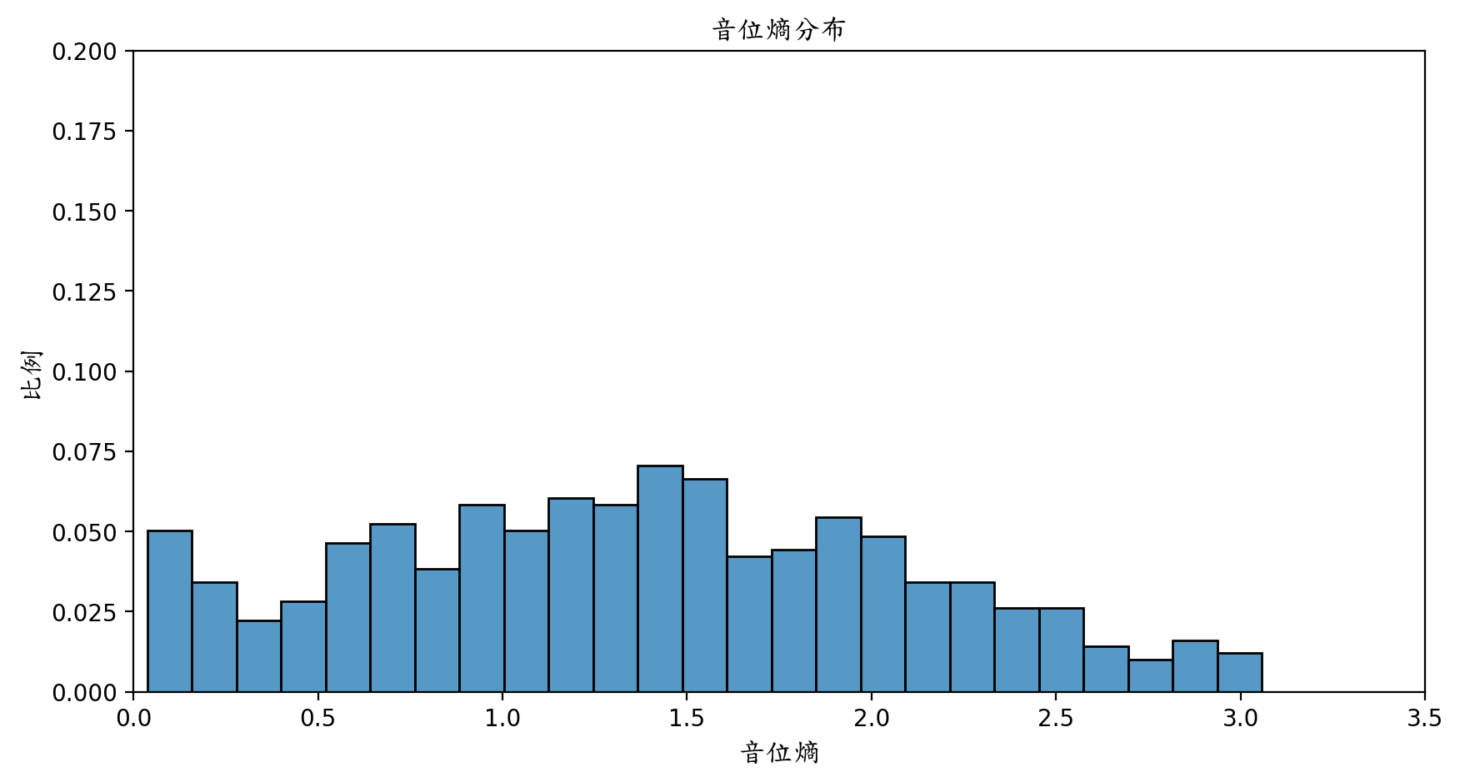
\includegraphics[width=\tempwidth]{feasiblefigs/ch4figs/hub-u100-ap0500-phnent-hist.png}
                 \caption{500 種次詞單位}
                 \label{fig:hub-u100-ap0500-phnent-hist}
             \end{subfigure}
             \vfill
             \begin{subfigure}{\textwidth}
                 \centering
                 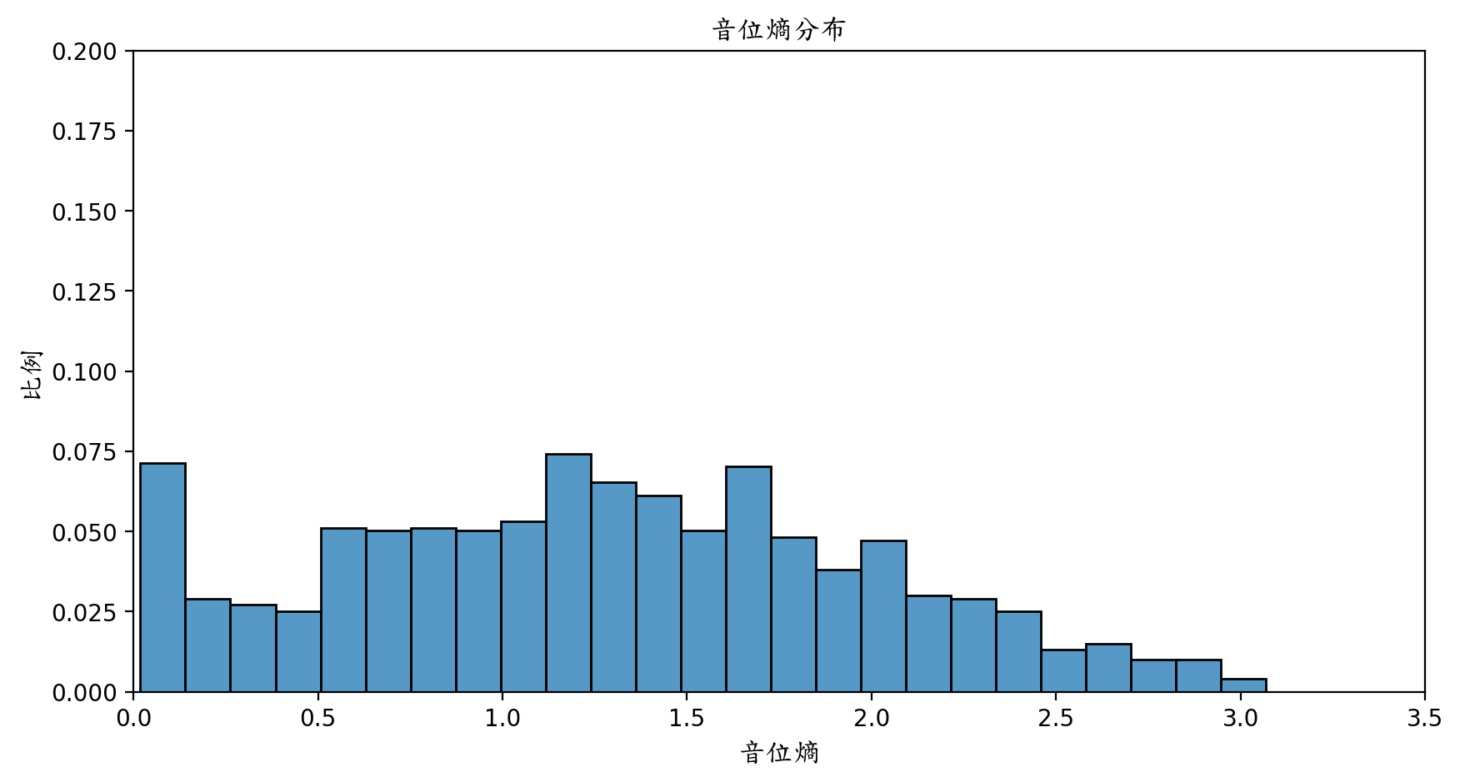
\includegraphics[width=\tempwidth]{feasiblefigs/ch4figs/hub-u100-ap1000-phnent-hist.png}
                 \caption{1000 種次詞單位}
                 \label{fig:hub-u100-ap1000-phnent-hist}
             \end{subfigure}

             \caption{HuBERT 表徵在 K-平均演算法使用分群數 100 後,}
             比較不同次詞單位數量的音位條件熵 $H(y|z)$ 直方圖
             \label{fig:hub-u100-hist-comparisons}
        \end{figure}
    }
}


  首先,考慮不同聲學片段數量對於機率熱圖與純度數據的影響。從圖 \ref{fig:hub-u050-comparisons} 與圖 \ref{fig:hub-u100-comparisons} 分別比較了不同聲學片段的機率熱圖,它們分別是 HuBERT 模型配合分群數為 50 和 100 的離散單元模型,並將各自的離散單元使用單一詞演算法得到次詞單位數量為 500 和 1000 的聲學片段所得到的結果。\par
        從中我們可以看出,當聲學片段數量上升時,由於有了更多的符記可以讓離散表徵區別更細節的發音差異,因此整體的純度數值有所提升。從熱圖上也可以觀察出更深的色塊,也就是有了更多的符記可以集中的對應到特定音位。然而,由於符記數量的上升,機率熱圖整體也變得更加碎片化,因此歸類同樣音位的效果也相對變得較不明顯。\par
        為了確認每個聲學片段對應音位之集中狀況,我們可以觀察音位熵的直方圖變化。一樣比較 HuBERT 模型、K-平均分群數 50 和 100 在使用 500 和 1000 個次詞單位得到的聲學片段所對應的音位條件熵 $H(y|z)$ 的直方圖,呈現在圖 \ref{fig:hub-u050-hist-comparisons} 與圖 \ref{fig:hub-u100-hist-comparisons} 中,可以看出,透過分詞方法的引入,相比於尚未使用的單一離散單元進行的統計數據,改用聲學片段可以讓整體的音位熵確實降低,亦即各自符記對應的音位變得更加明確,與我們從機率熱圖上所觀察到的趨勢符合。\par
        雖然改用聲學片段會使熱圖的對應規律變得更加複雜而難以觀察,但除純度與相互資訊的數值變化外,從符記代表性音位的比例變化,也可以驗證更多的符記可以區別發音細節這點。我們回到圖 \ref{fig:hub-u050-comparisons} 中觀察 HuBERT 在分群數 50 時的機率熱圖,圖中的藍色鉛直線是每個聲學片段按對應音位之分類,排序分區的結果。因此觀察藍色鉛直線在橫軸上各區的比例變化,可以理解這些符記以多少的比例對應不同音位的發音特徵。第三章在單一離散單元分群數為 50 時,由於離散單元數較少,並沒有任何單元最高機率對應塞擦音音位。然而,當對這些離散單元進行分詞處理後,不管在次詞單位數量為 500 或 1000 的機率熱圖上,都可以看見出現了至少一個符記可以對應到塞擦音,由此驗證藉由引入分詞方法提升次詞單位數量,對捕捉更細微的發音差異的確是有所幫助的。


\subsubsection{原先離散單元分群數對聲學片段的影響}


{
    {
        \begin{figure}
             \centering
             \begin{subfigure}{\textwidth}
                 \centering
                 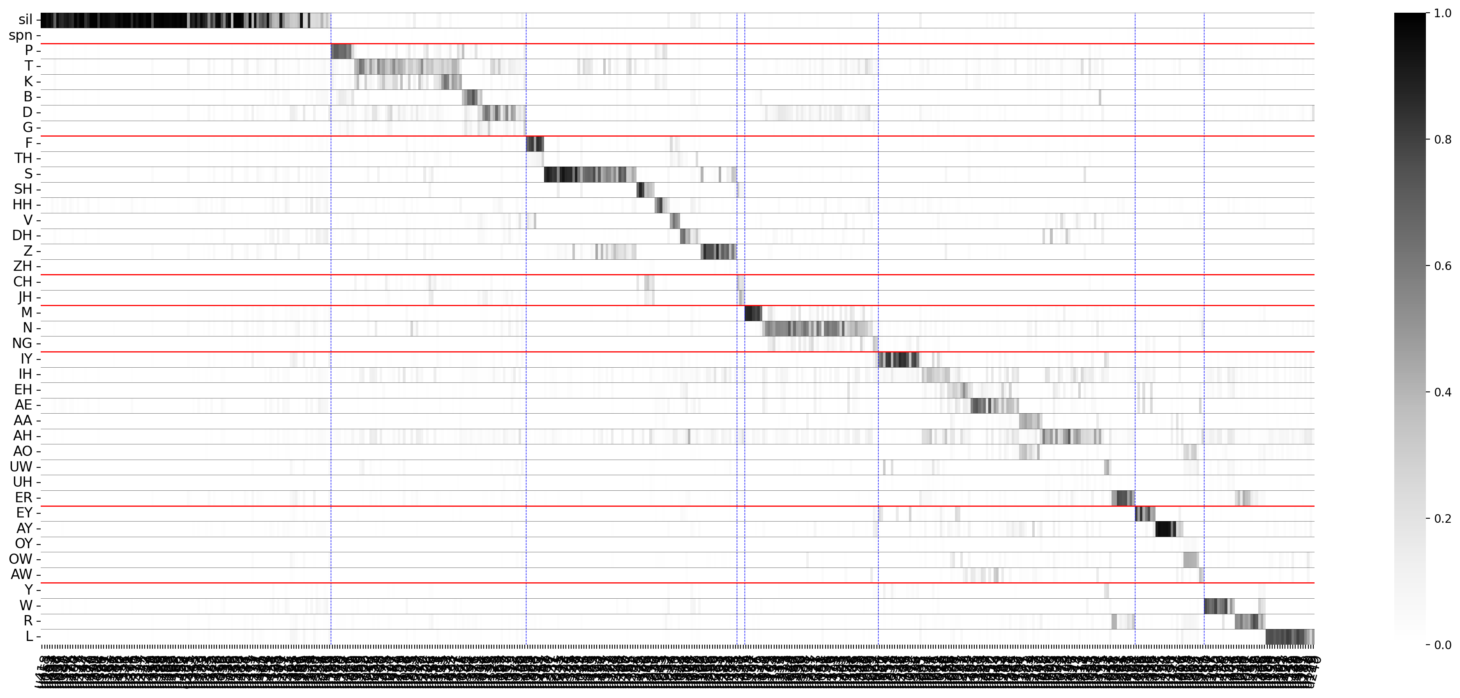
\includegraphics[width=1\linewidth]{feasiblefigs/ch4figs/hub-u050-ap0500-givenunit-byphn.png}
                 \caption{分群數 50}
                 \label{fig:hub-u050-ap0500-givenunit-byphn--picked}
             \end{subfigure}
             \vfill
             \begin{subfigure}{\textwidth}
                 \centering
                 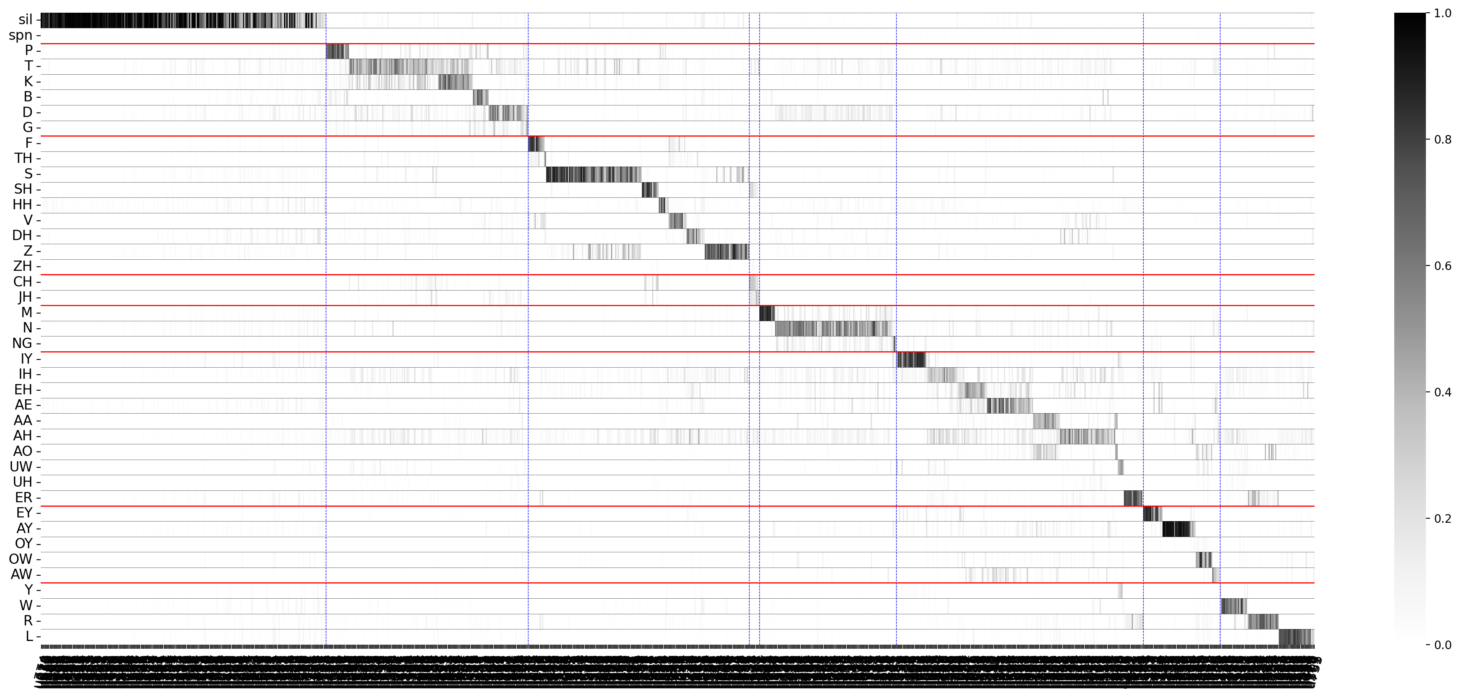
\includegraphics[width=1\linewidth]{feasiblefigs/ch4figs/hub-u050-ap1000-givenunit-byphn.png}
                 \caption{分群數 100}
                 \label{fig:hub-u100-ap0500-givenunit-byphn--picked}
             \end{subfigure}
             \caption{比較同樣 500 種次詞單位的聲學片段模型,著重比較 HuBERT 表徵}
             在 K-平均演算法使用分群數 50 與 100 的條件機率熱圖 $p_{y|z}(i|j)$ 差異
             \label{fig:check-ap0500}
        \end{figure}
    }
}



  然而,儘管分詞方法的引入在一定程度上幫助了區別語音訊號中的細微發音差異,若要更直接的對這件事進行改善,在原始的語音表徵進行 K-平均演算法離散化時,其分群數仍為了更關鍵的決定因素。圖 \ref{fig:check-ap0500} 比較了同樣次詞單位數量為 500 時,離散表徵分群數為 50 和 100 的機率熱圖差異,可以發現分群數為 100 的機率熱圖能更加平均的對應到不同的音位,而不如分群數 50 的機率熱圖對於某些音位的捕捉效果那麼不平均。然而,即便對音位標註的歸類效果最大的取決於離散單元分群數,在遇到運算資源限制,使得使用大量分群數進行 K-平均演算法難以實行時,仍舊可以藉助分詞方法的引入提升整體表現。
        \jcm{藉由比較幾章機率熱圖的差異,我們可以確認這件事。 \jcm{補寫一下}}

        \jcm{
        
        我們這邊可以比較一下 50、100、50+100、50+500、100+500 的熱圖。從這邊可以驗證前面所說的:在基底分群數確定的情形之下,的確一開始分群數開得比較大,整體對語音規律的捕捉效果就會比較好,但藉由分群方法的引入,至少 50 分群數可以藉由符記數提升的機會,來重新編碼語音中的結構,也就是雖然不如 K-平均演算法那樣因為直接做用於語音表徵空間,那麼好區分出發音的差異,但藉由分詞演算法,仍然可以從捕捉語音中明顯重複的序列資訊\textcolor{red}{[這時候是不是要擺一下長度 & 常見 pattern 統計數據確認了?] } ,獲取語音序列中跟發音有關的特徵,進而模擬類似人類理解音位的過程。
        
        }
}

    {
        \newcommand{\tempwidth}[0]{0.8\linewidth}
        \begin{figure}
             \centering
             \begin{subfigure}{\textwidth}
                 \centering
                 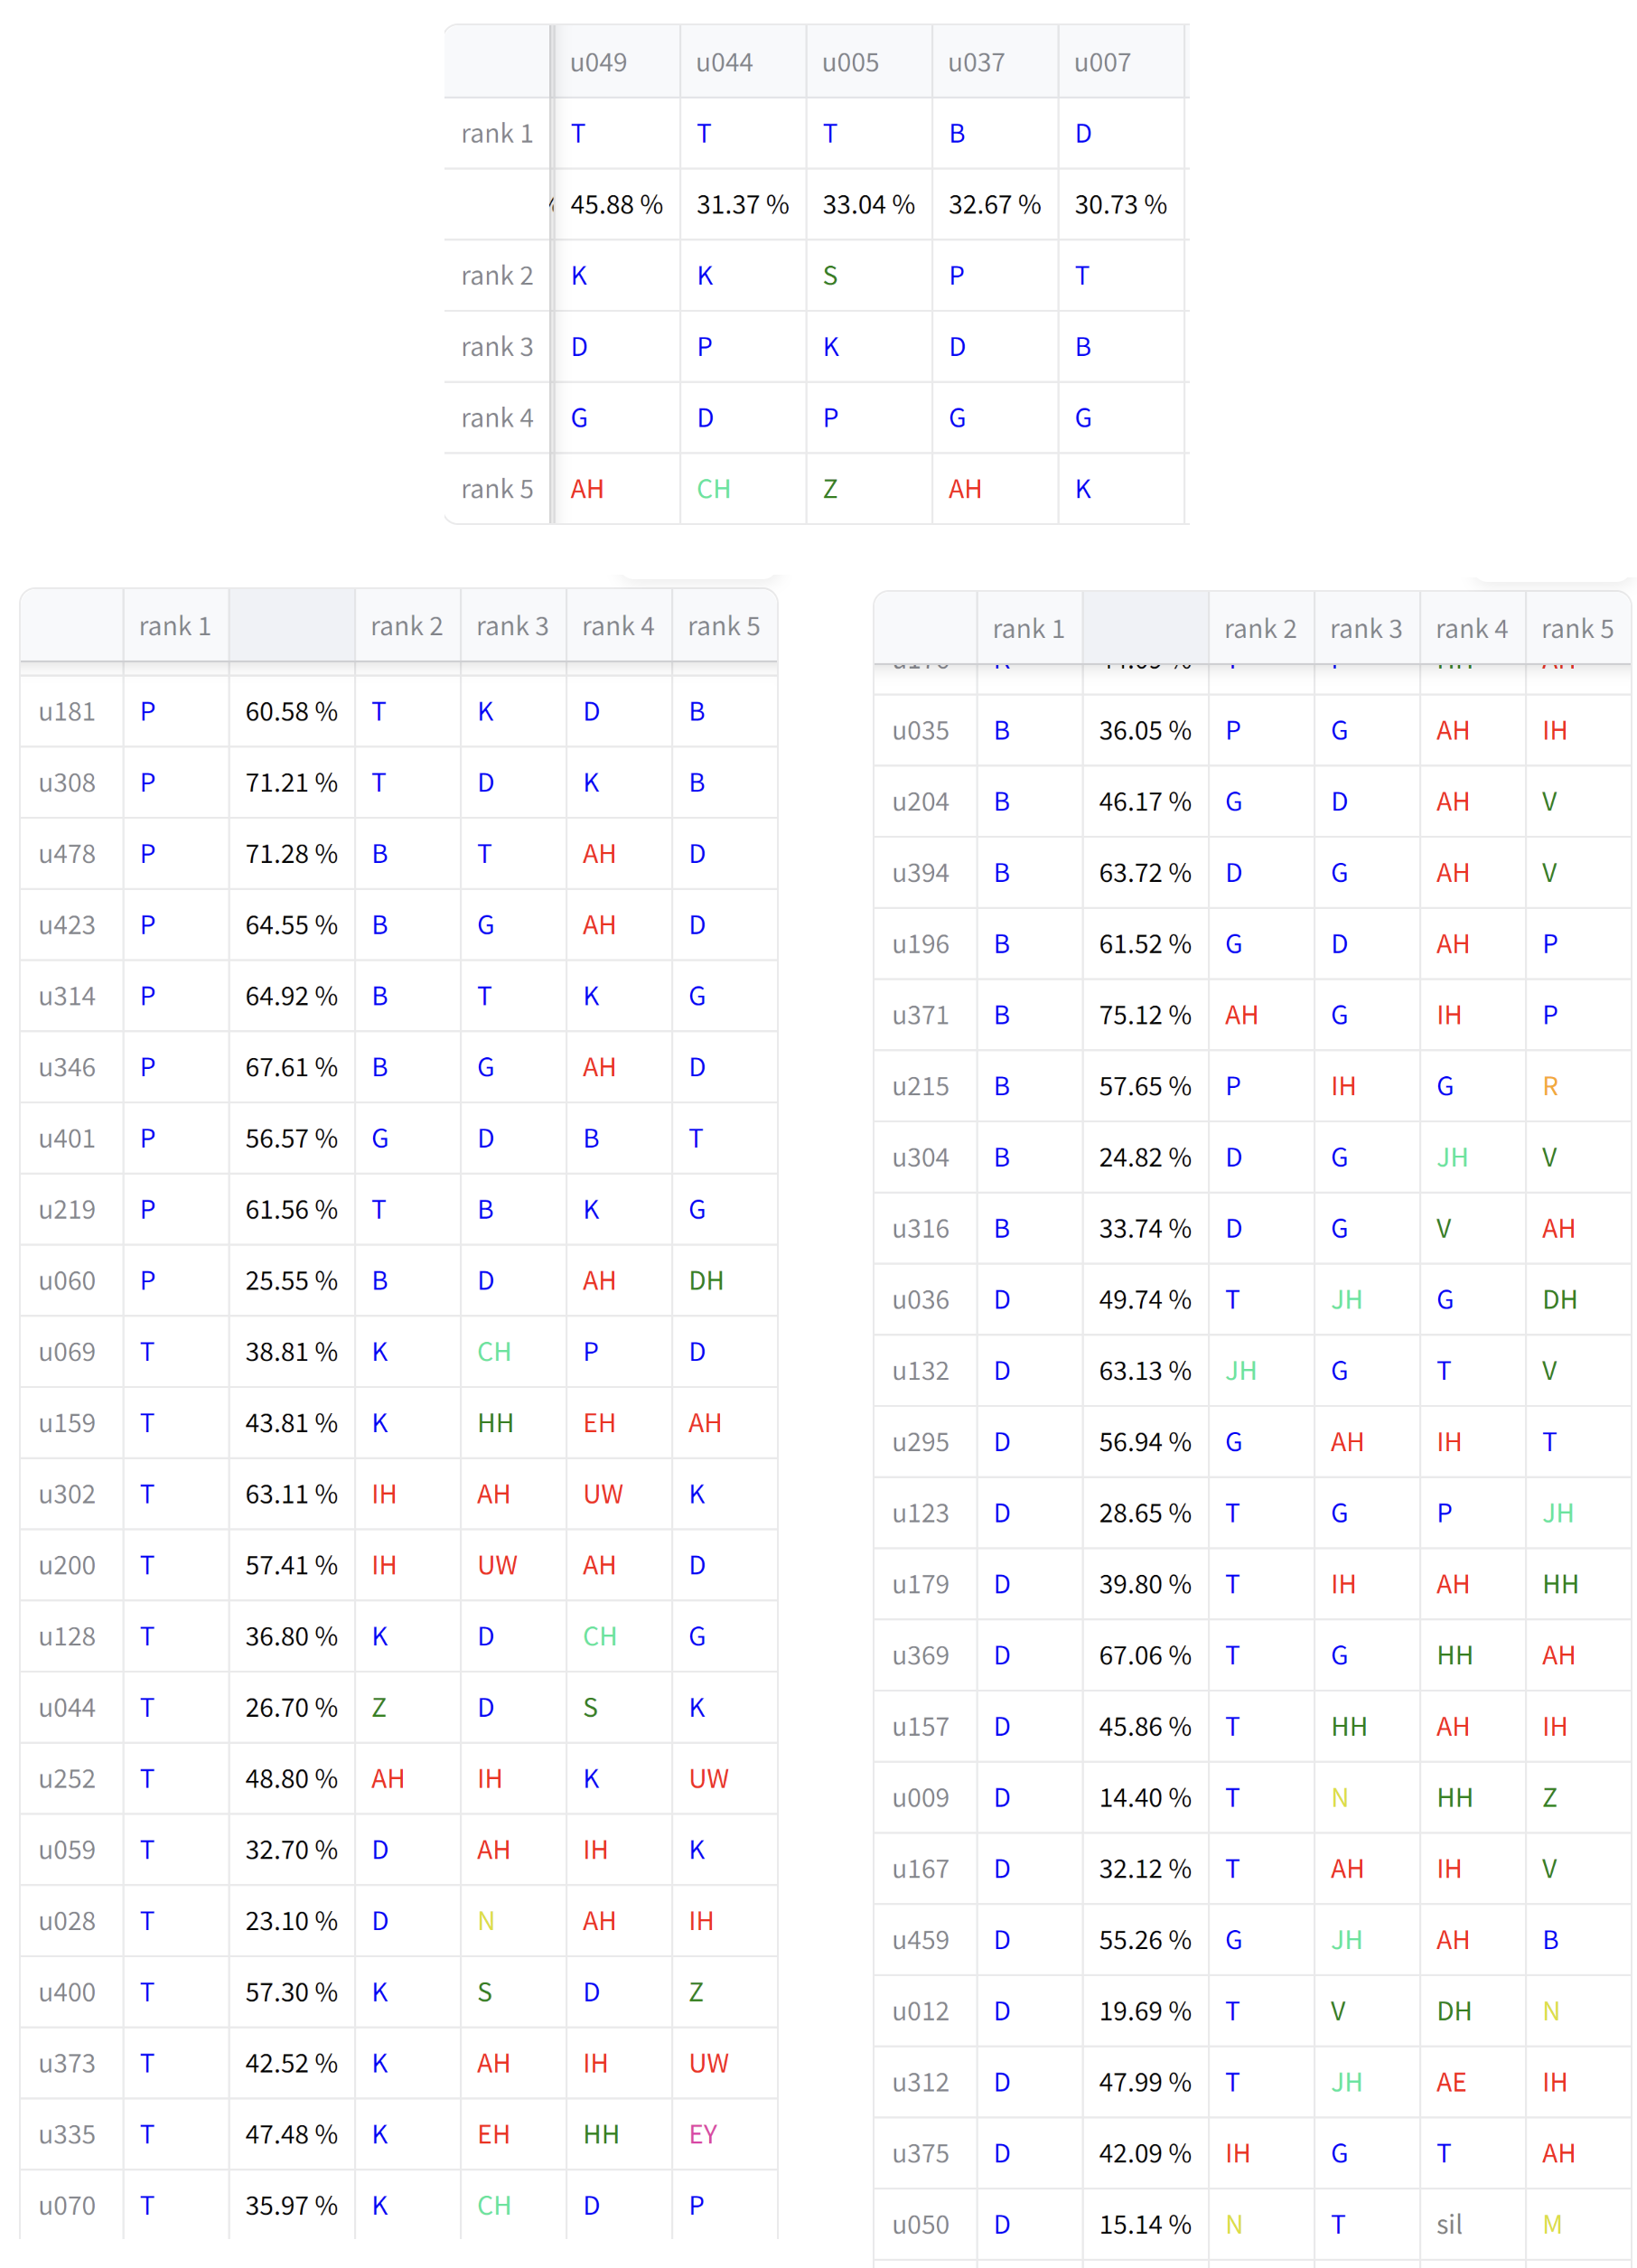
\includegraphics[width=\tempwidth]{chapters/plo_phn.png}
                 \caption{塞音}
                 \label{fig:hub-u050-ap0500-ploobs}
             \end{subfigure}
             \vfill
             \begin{subfigure}{\textwidth}
                 \centering
                 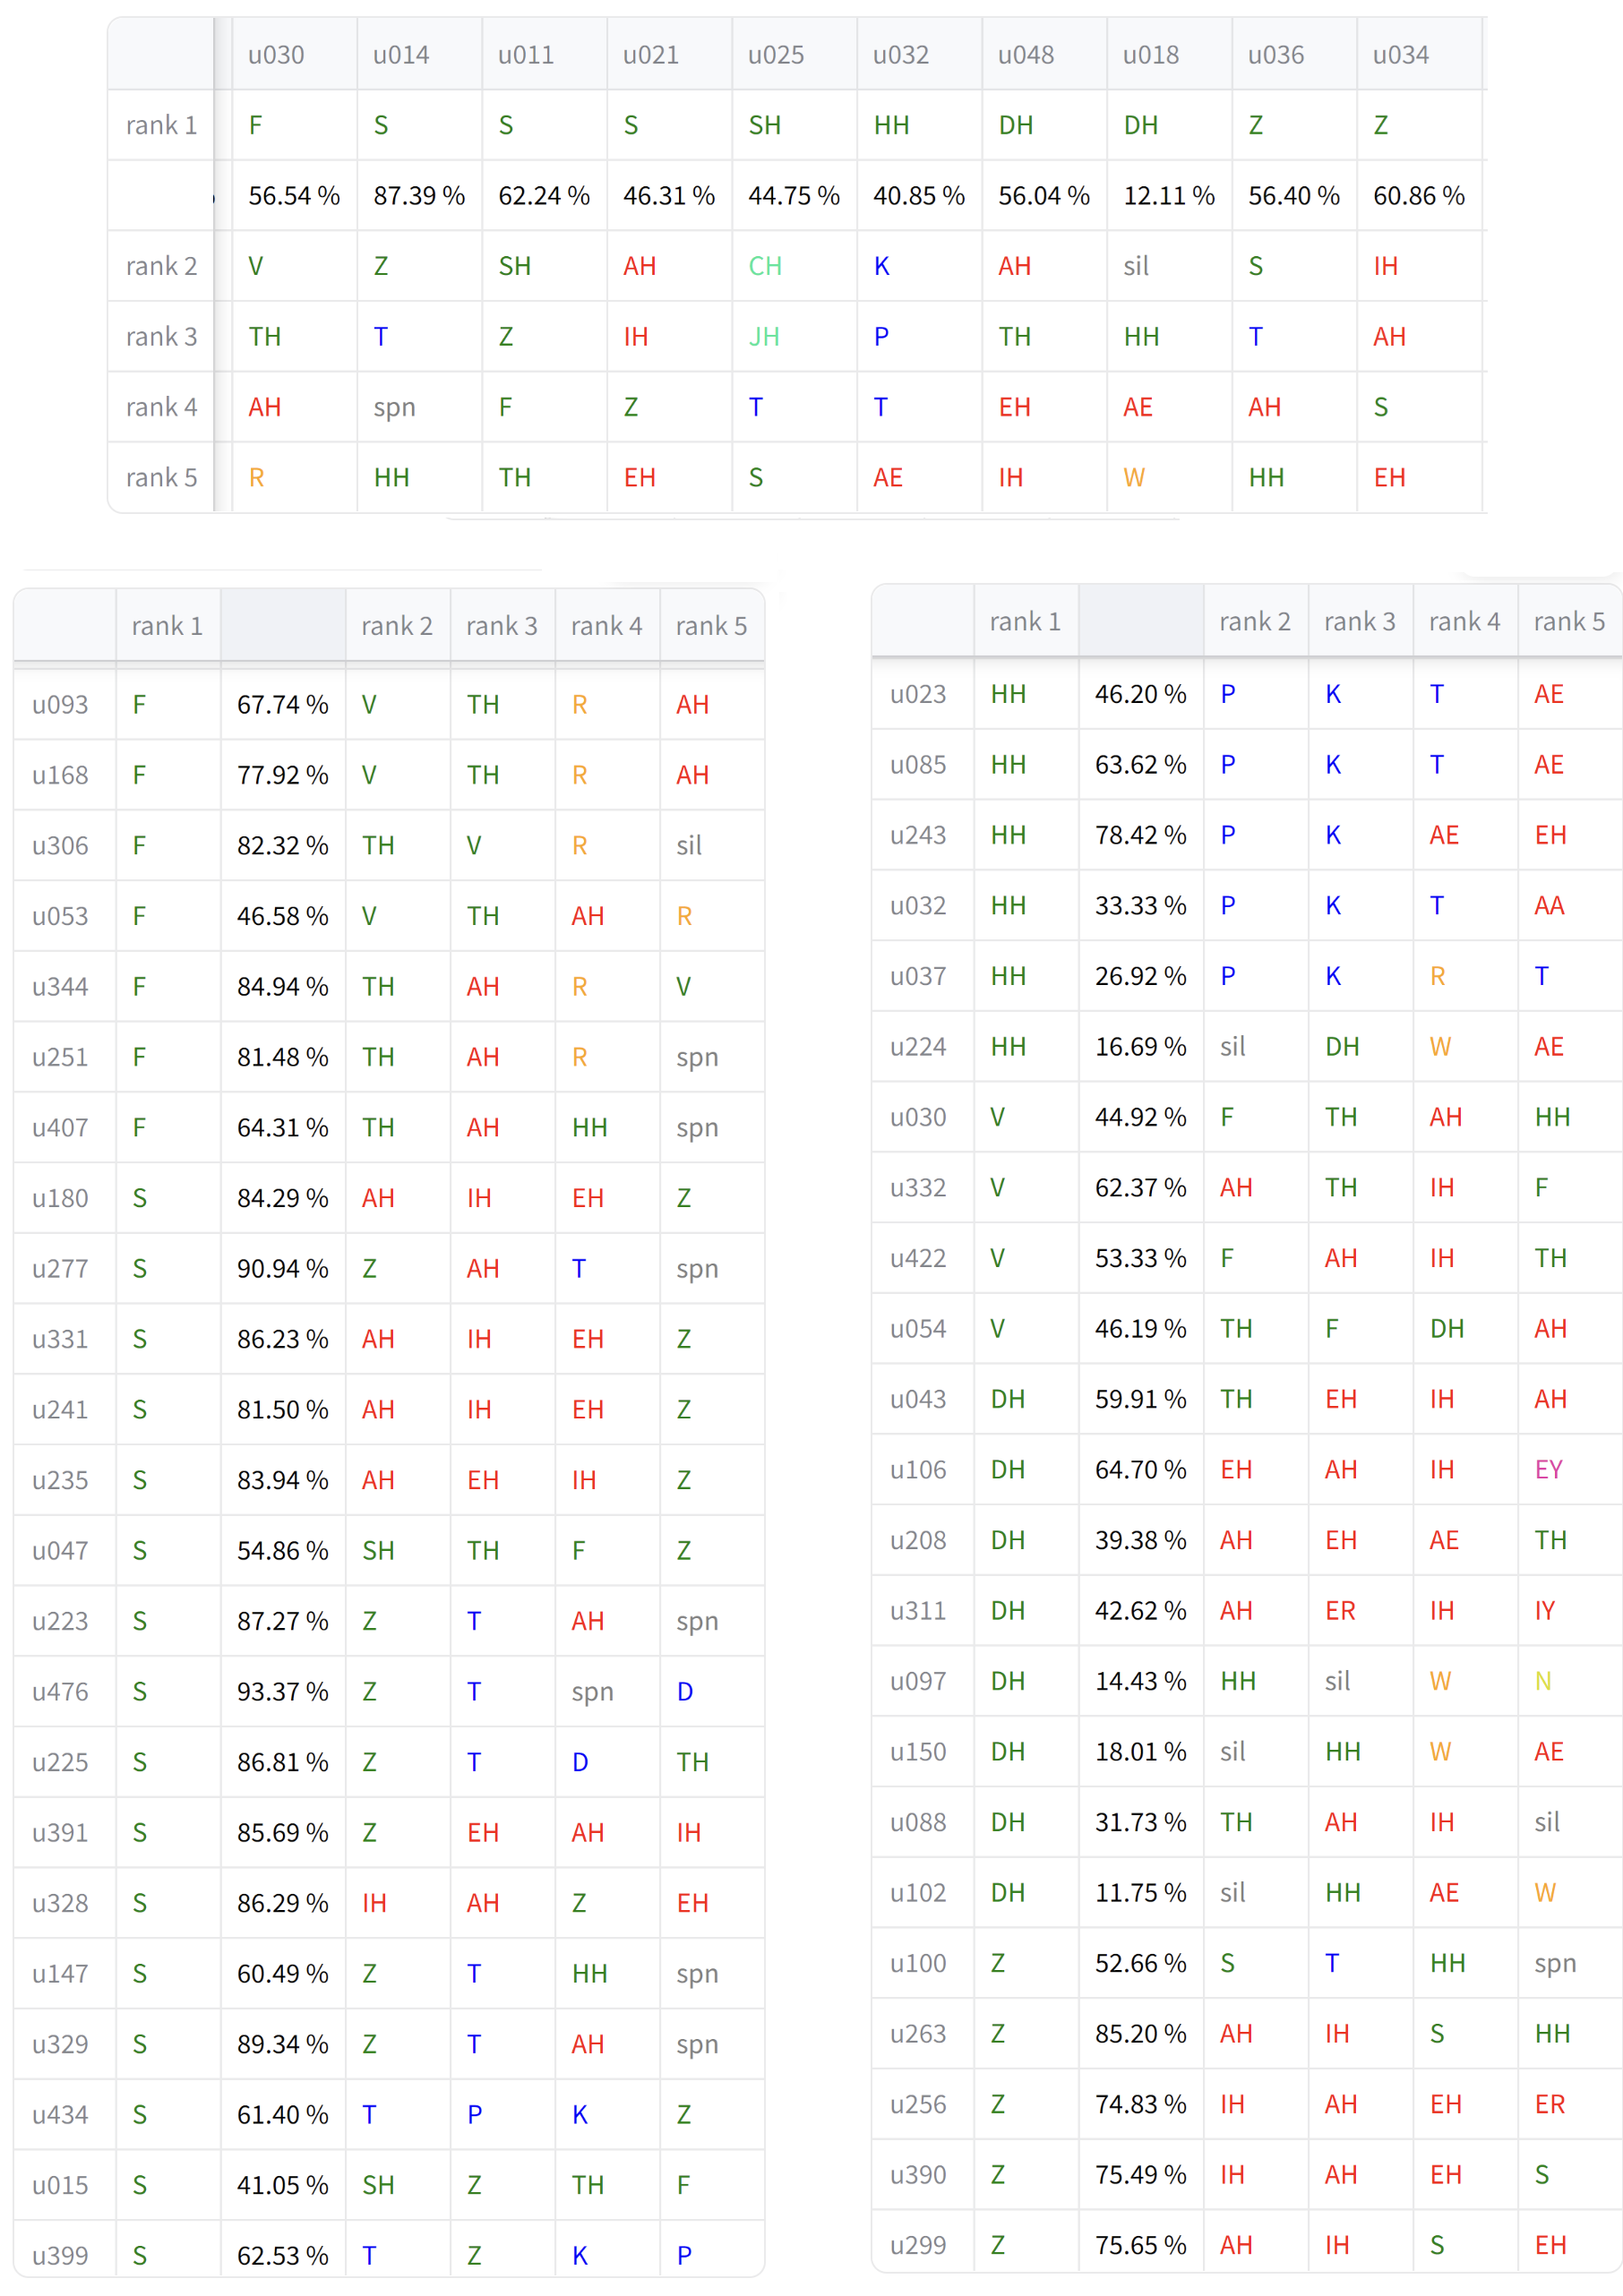
\includegraphics[width=\tempwidth]{chapters/fri_phn.png}
                 \caption{擦音}
                 \label{fig:hub-u050-ap0500-friobs}
             \end{subfigure}
             \vfill
             \begin{subfigure}{\textwidth}
                 \centering
                 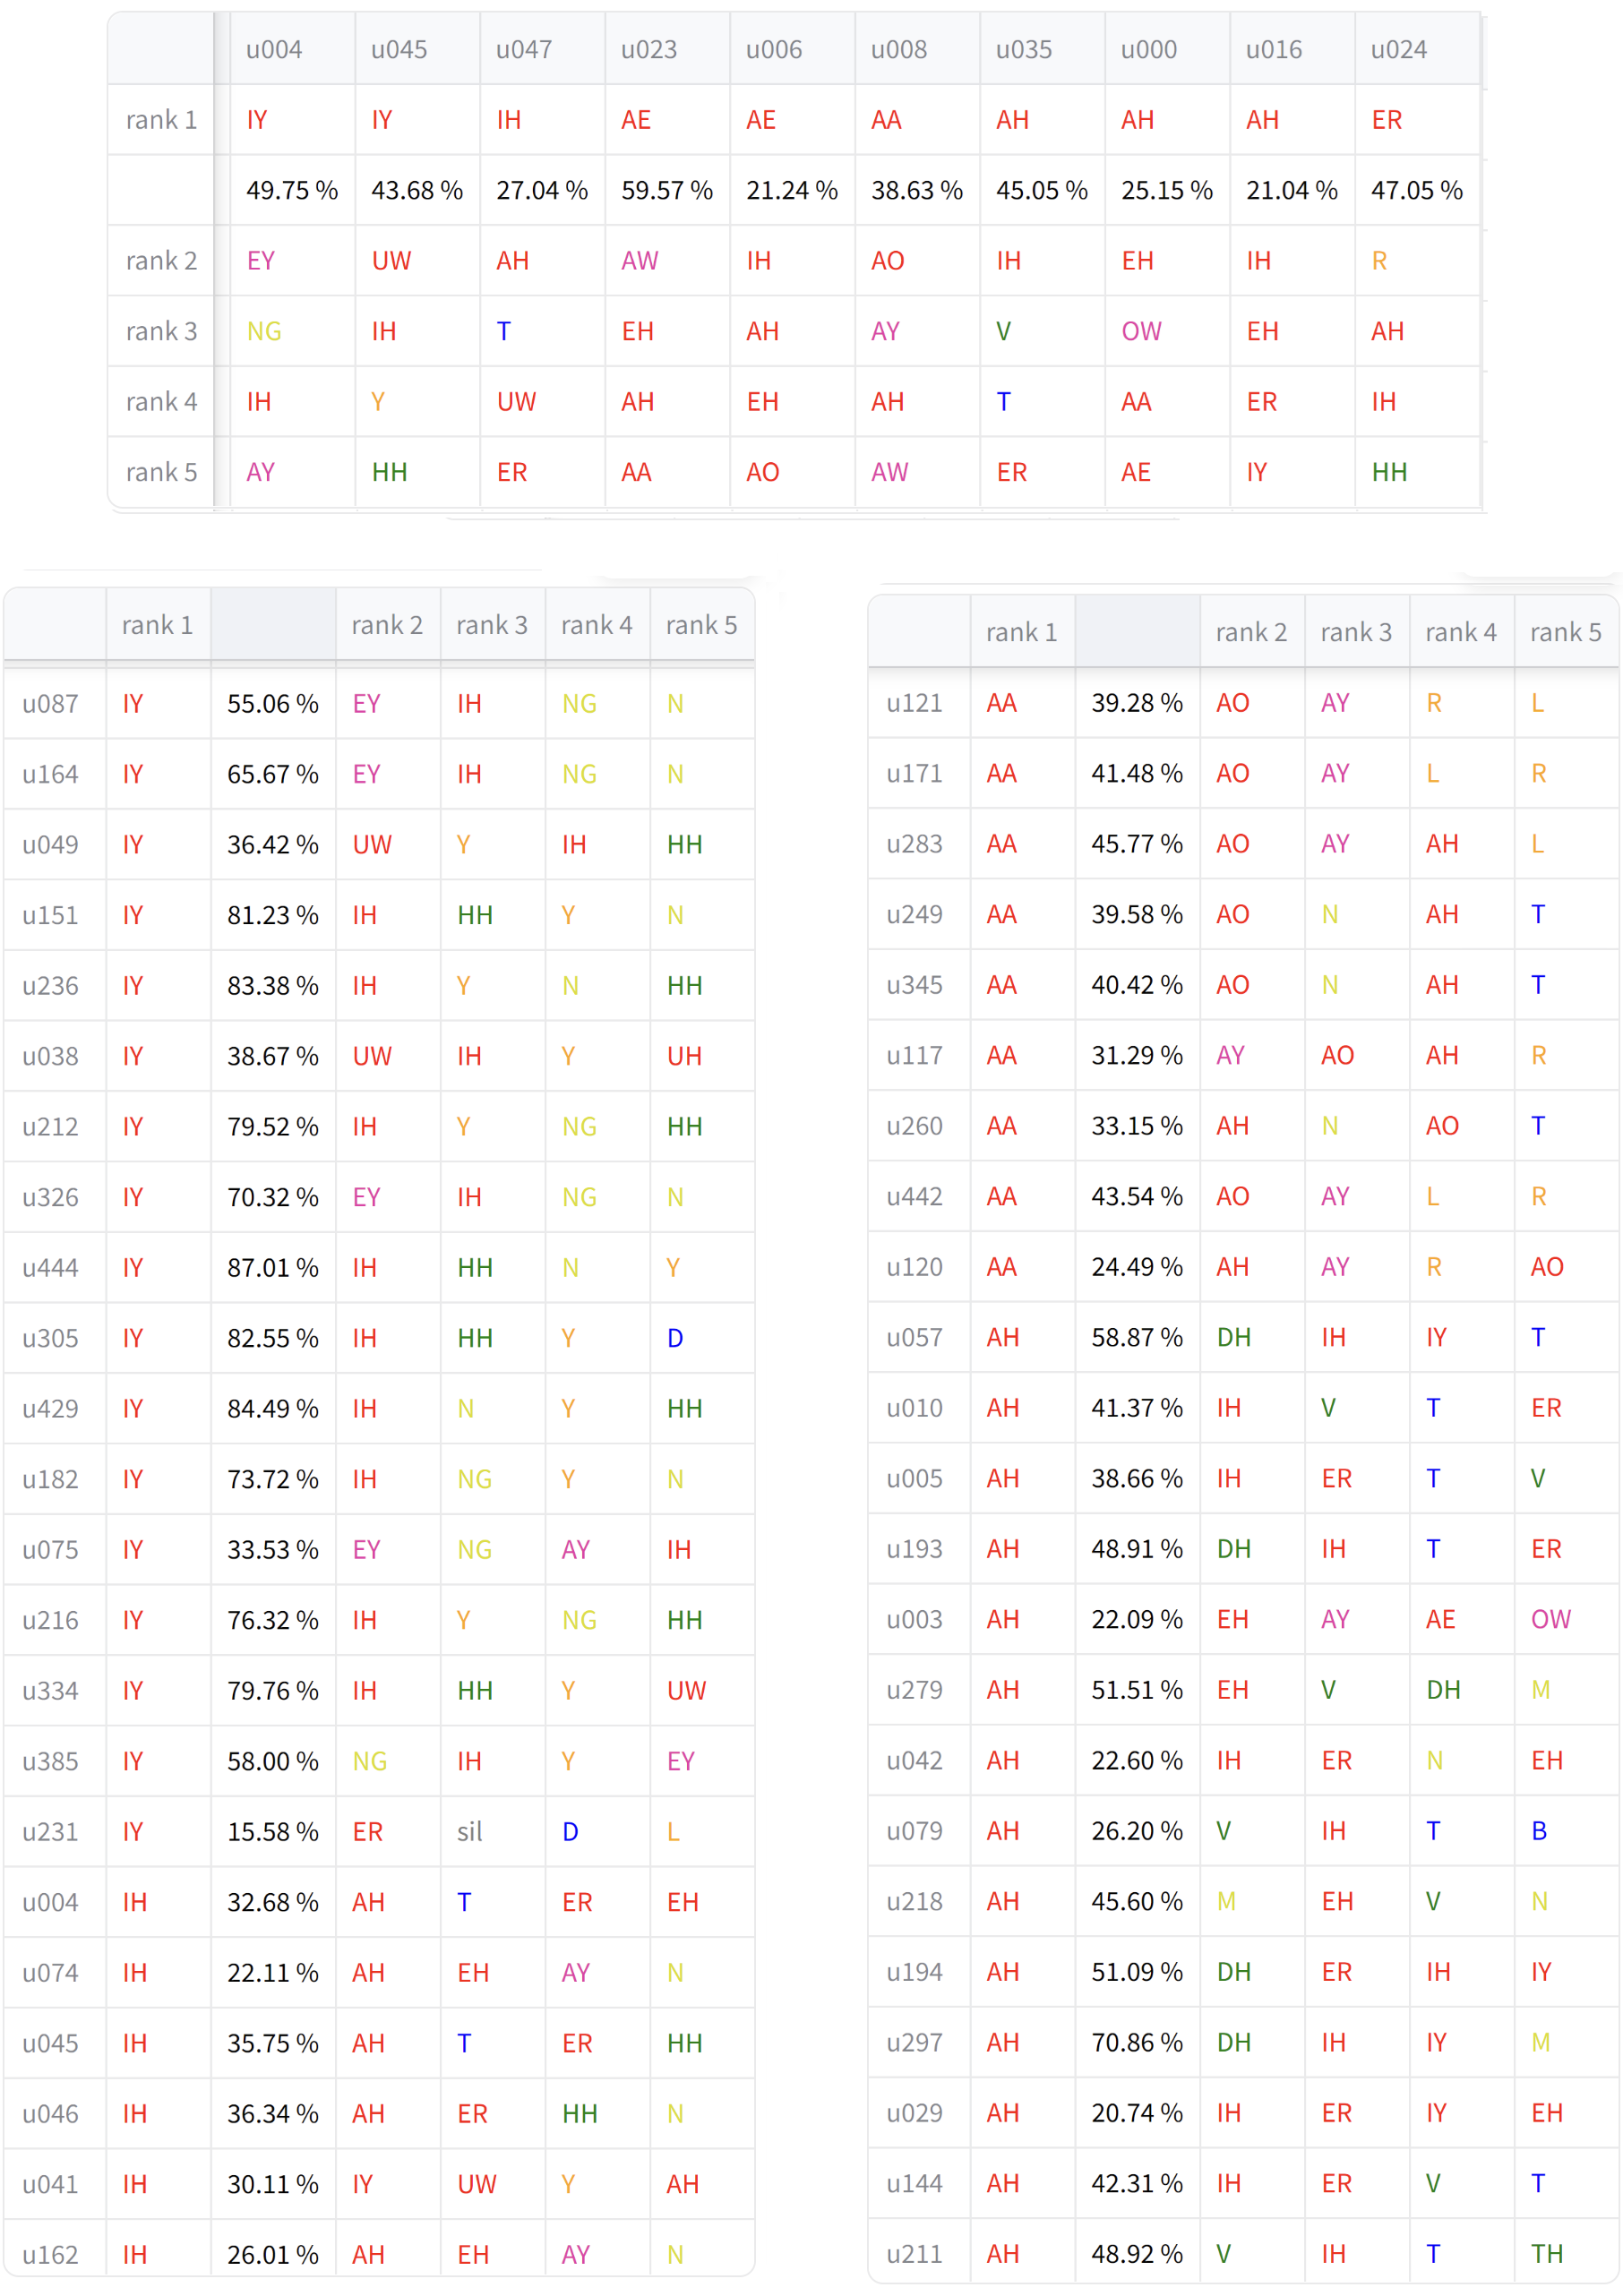
\includegraphics[width=\tempwidth]{chapters/vow_phn.png}
                 \caption{單元音}
                 \label{fig:hub-u050-ap0500-vowobs}
             \end{subfigure}

             \caption{HuBERT 表徵、K-平均演算法分群數 50,比較單一離散單元與使用 500 種次詞單位,}
             依據不同音位分類比較符記各自對應的前五高音位
             (上半部為離散單元,下半部為聲學片段。圖中的百分比為最高機率音位的條件機率 $p_{y|z}(i^*(j)|j)$)
                         \label{fig:hub-u050-phnobserver}
        \end{figure}
    }

\begin{figure}
    \centering
    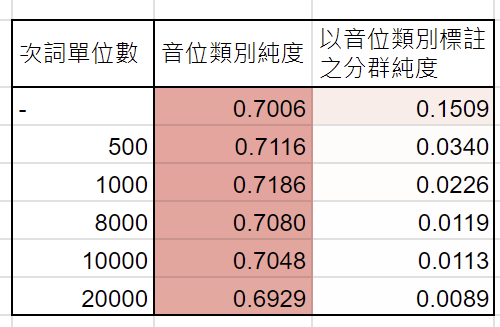
\includegraphics[width=0.5\linewidth]{.vscode/hub50clspur.png}
    \caption{Enter Caption}
    \label{fig:enter-label}
\end{figure}

\begin{figure}
    \centering
    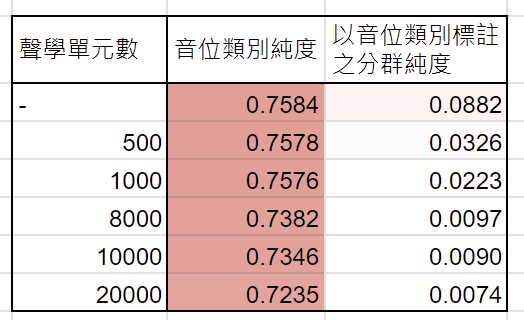
\includegraphics[width=0.5\linewidth]{hub100pcs--clupur.png}
    \caption{Enter Caption}
    \label{fig:enter-label}
\end{figure}
\subsubsection{各自離散單元視角的切入}
  接下來,我們也可以如同第三章對各自離散單元視角切入,觀察各個聲學片段對應音位之間的混淆關係,也就是對應機率前幾高音位之間是否依然如離散單元那樣存在特定特徵。圖 \ref{fig:hub-u050-phnobserver} 為 HuBERT 分群數 50 後取 500 個次詞單位所得聲學片段中,部分次詞單位所對應前五高機率音位對應排名,其中特別將塞音、擦音和單元音拿出來比較。圖中的上半部是離散單元,下半部則是聲學片段。從中可以發現,比起離散單元,由於聲學片段的符記數量更多,因此在維持對應音位之間相關性的同時,卻可以呈現出不同音位更細節的相關性。例如在圖 \ref{fig:hub-u050-ap0500-ploobs} 中,上半部顯示原先在離散單元時因為只有 50 個符記種類,因此只能看出 T、B 與 D 比較容易和哪些其他音位比較相關;但聲學片段卻可以呈現出 P、T、B、D 等更多細節的音位關係。
    (aff 圖)
    \begin{figure}
        \centering
        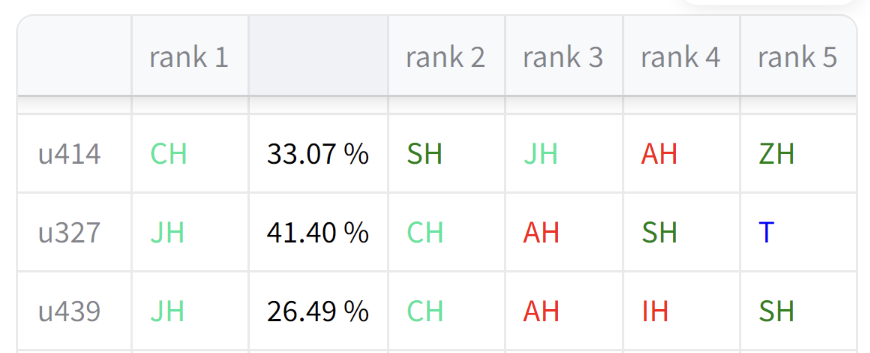
\includegraphics[width=0.5\linewidth]{chapters/aff-hub50-500.png}
        \caption{Enter Caption}
        \label{fig:aff}
    \end{figure}


        仿照第三章,我們也可以從「用音位分類為新標籤計算的純度」數據來證明這件事。隨著詞表大小的上升,整體的音位分類標註純度卻只有些微提升,而且愈來愈不明顯,幾乎沒什麼提升的空間了。 \par
        這很可能是因為分詞演算法本身的特性,聲學片段可以把帶有不同代表性音位的離散單元合在一起,因此整體對特定音位的代表性跟語音相關性就低上了不少。  \jcm{phn pur up, but pcls pur down}

\subsection{以音位角度切入}

\begin{figure}
    \centering
    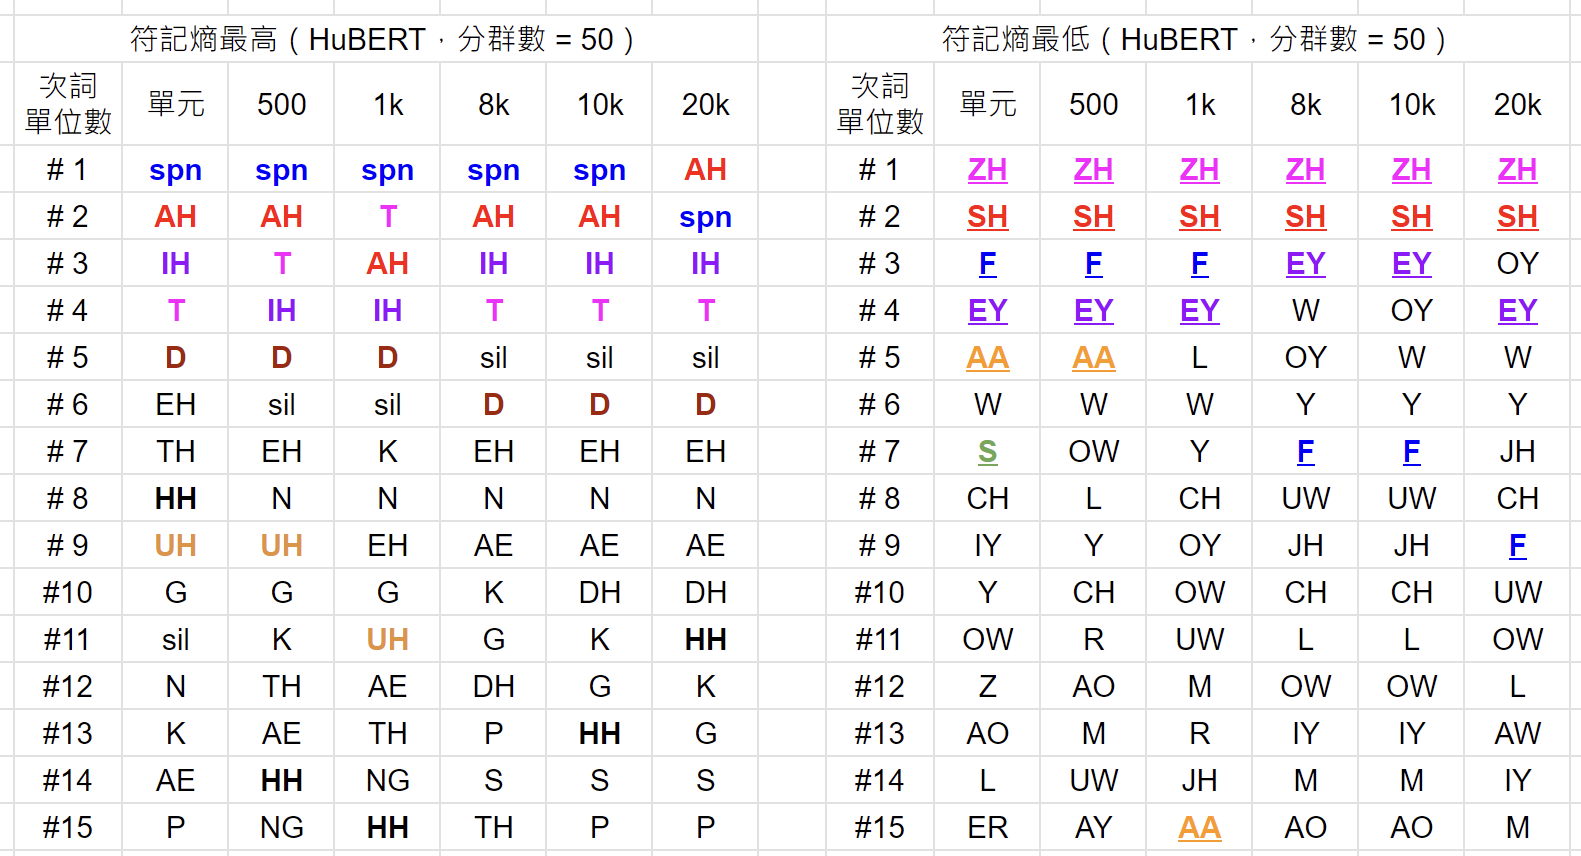
\includegraphics[width=0.5\linewidth]{phnrank-hub50pcs.png}
    \caption{Enter Caption}
    \label{fig:enter-label}
\end{figure}

\begin{figure}
    \centering
    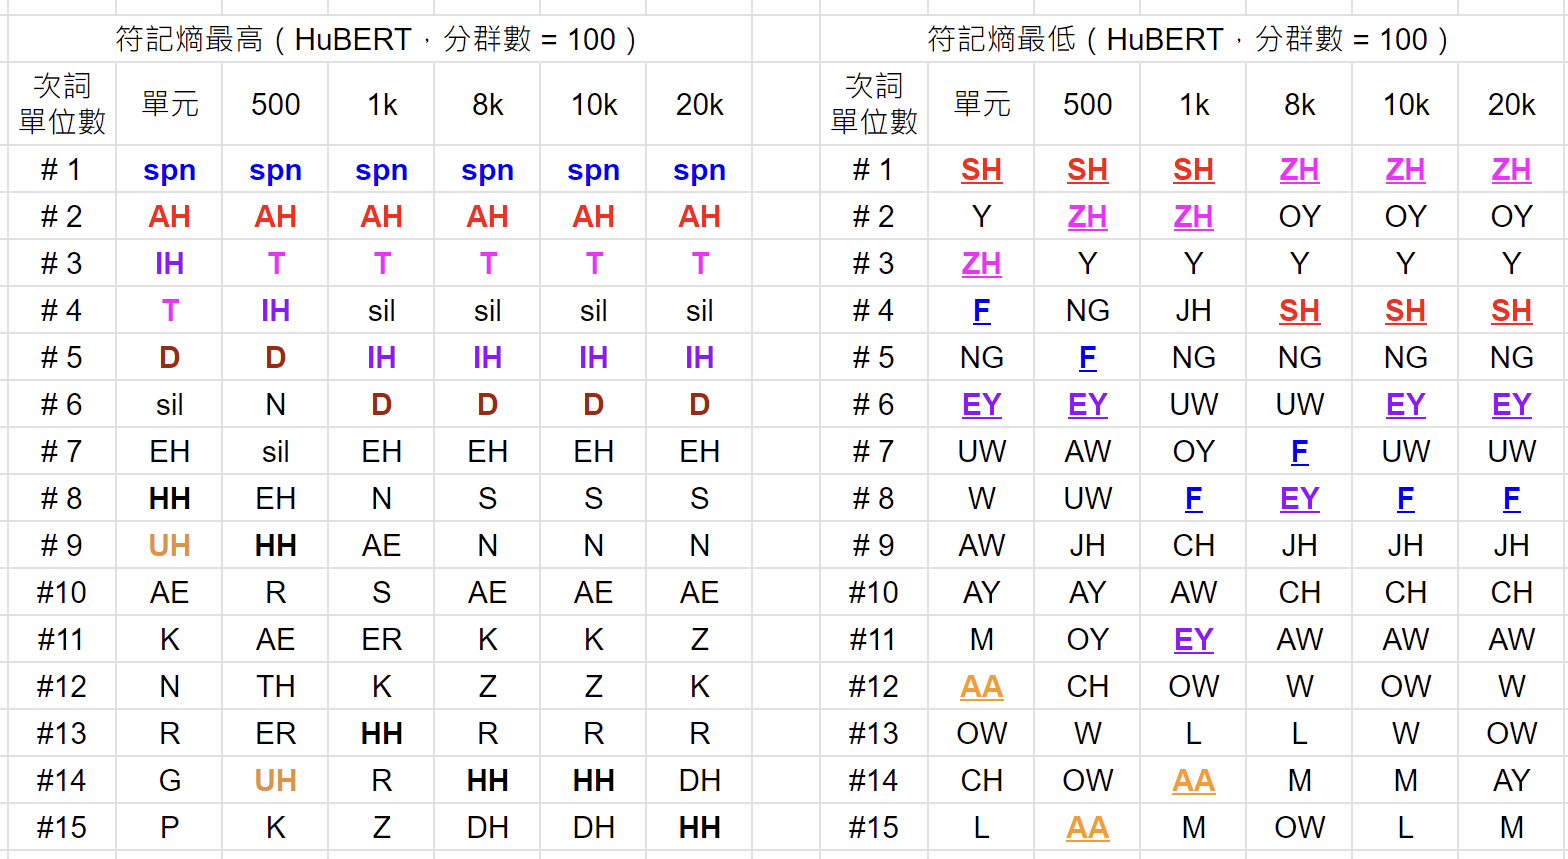
\includegraphics[width=0.5\linewidth]{phnrank-hub100pcs.png}
    \caption{Enter Caption}
    \label{fig:enter-label}
\end{figure}
  接著,我們轉而再度去以音位的角度切入,觀察各自音位的符記分佈集中程度。從圖 \ref{005} 中我們可以看到,整體排名趨勢幾乎與第三章不做分詞時的排名差不多,推論音位本身的容易或難以歸類的特性,單靠對語音表徵進行分群就已經可以不錯的發現這些現象。然而,即便分詞方法本身有機率將不同代表性音位的離散單元重新合在一起,卻也仍然大致維持了這個趨勢。因此,我們可以推論,音位本身對應符記的分散程度,不論是使用 K-平均演算法離散化,或是用分詞方法重新歸類次詞單位得到,這個分散程度的趨勢都是差不多的,音位本身的發音特徵或許是一個超出音框本身、影響範圍更廣泛的特性。 \par




{
\begin{figure}
    \centering
    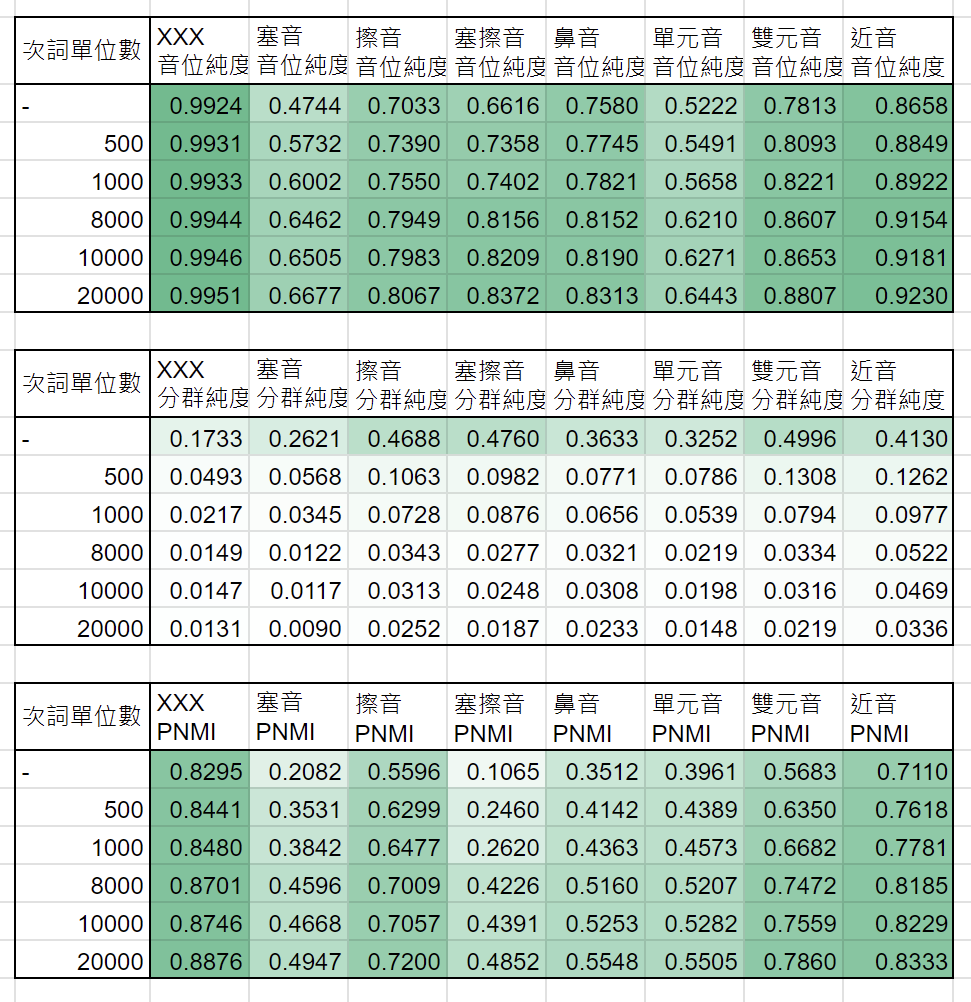
\includegraphics[width=0.5\linewidth]{hub50-ap-detailedpur.png}
    \caption{Enter Caption}
    \label{fig:hub50-ap-detailedpur}
\end{figure}
}


\begin{figure}
    \centering
    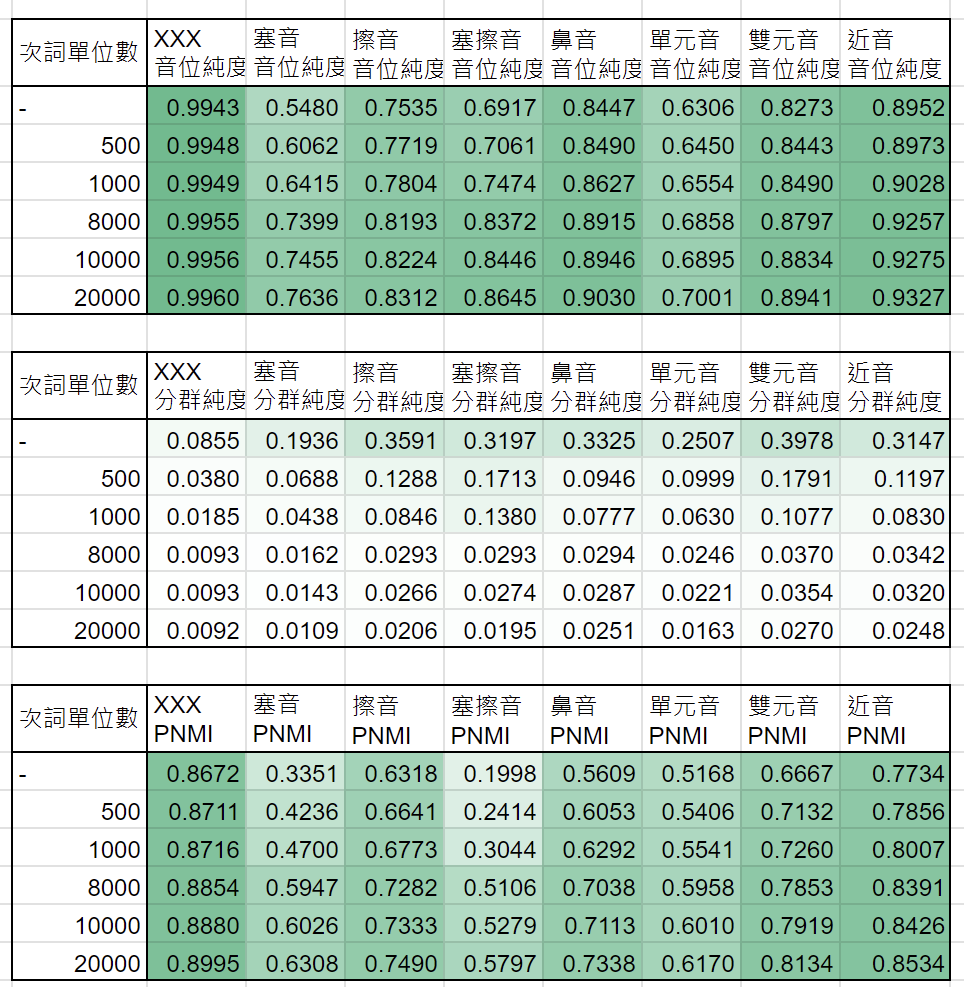
\includegraphics[width=0.5\linewidth]{hub100-ap-detailedpur.png}
    \caption{Enter Caption}
    \label{fig:hub100-ap-detailedpur}
\end{figure}


  
        最後,我們可以統計一下各音位分類的純度與相互資訊數據,與上一章節比對。由圖 \ref{fig:hub50-ap-detailedpur} 中可以看到,除了原本純度較低的塞音比較有所提升以外,其他純度較高的音位分類純度提升得很有限。儘管很不明顯,但整體大致仍然是有所提升的。

{

{
\begin{table}[!htbp]
    \centering
    \begin{subtable}[t]{\textwidth}
        \centering
        \begin{tabular}{|c|c|c|c|c|c|c|} \hline 
                詞表大小  & 音位純度 & 分群純度 & 音位熵 & 離散單元熵 &    PNMI & 長度壓縮比率 \\ \hline 
50 (未分詞)& 0.5256& 0.3382& 3.3152& 3.8681& 0.4993&1.0000\\ \hline 
                   500  &   0.5574   &  0.0829 &   3.3152  &  6.0282 & 0.5357 & 0.3486  \\ \hline %%  1.7758       
                  1000  &   0.5744   &  0.0556 &   3.3152  &  6.6594 & 0.5466 & 0.2992  \\ \hline %%  1.8120       
                  8000  &   0.5957   &  0.0257 &   3.3152  &  8.5192 & 0.5729 & 0.2074  \\ \hline %%  1.8993       
                 10000  &   0.5955   &  0.0238 &   3.3152  &  8.7207 & 0.5750 & 0.2007  \\ \hline %%  1.9063       
                 20000  &   0.5921   &  0.0182 &   3.3152  &  9.3527 & 0.5820 & 0.1819  \\ \hline %%  1.9293       
        \end{tabular}
\caption{群數 = 50}
        \label{tab:ch4-hubert-phn-clu050}
    \end{subtable}        
    \jefftablesep        
    \begin{subtable}[t]{\textwidth}
        \centering
        \begin{tabular}{|c|c|c|c|c|c|c|} \hline 
                詞表大小  & 音位純度 & 分群純度 & 音位熵 & 離散單元熵 &    PNMI & 長度壓縮比率 \\ \hline 
100 (未分詞)& 0.6097& 0.2553& 3.3152& 4.5704& 0.5786&1.0000\\ \hline 
                   500  &   0.6260   &  0.0972 &   3.3152  &  6.0655 & 0.5990 & 0.4432  \\ \hline %%  1.9858       
                  1000  &   0.6372   &  0.0631 &   3.3152  &  6.7181 & 0.6089 & 0.3666  \\ \hline %%  2.0186       
                  8000  &   0.6536   &  0.0237 &   3.3152  &  8.5954 & 0.6308 & 0.2444  \\ \hline %%  2.0912       
                 10000  &   0.6527   &  0.0219 &   3.3152  &  8.7938 & 0.6324 & 0.2357  \\ \hline %%  2.0965       
                 20000  &   0.6490   &  0.0173 &   3.3152  &  9.4123 & 0.6378 & 0.2123  \\ \hline %%  2.1145       
        \end{tabular}
\caption{群數 = 100}
        \label{tab:ch4-hubert-phn-clu100}
    \end{subtable}        


\caption{HuBERT 模型在不同詞表大小時的音位分析數據}
    \label{tab:hubert-phn-results}
\end{table}

}  % tables
{

\begin{figure}
    \centering
    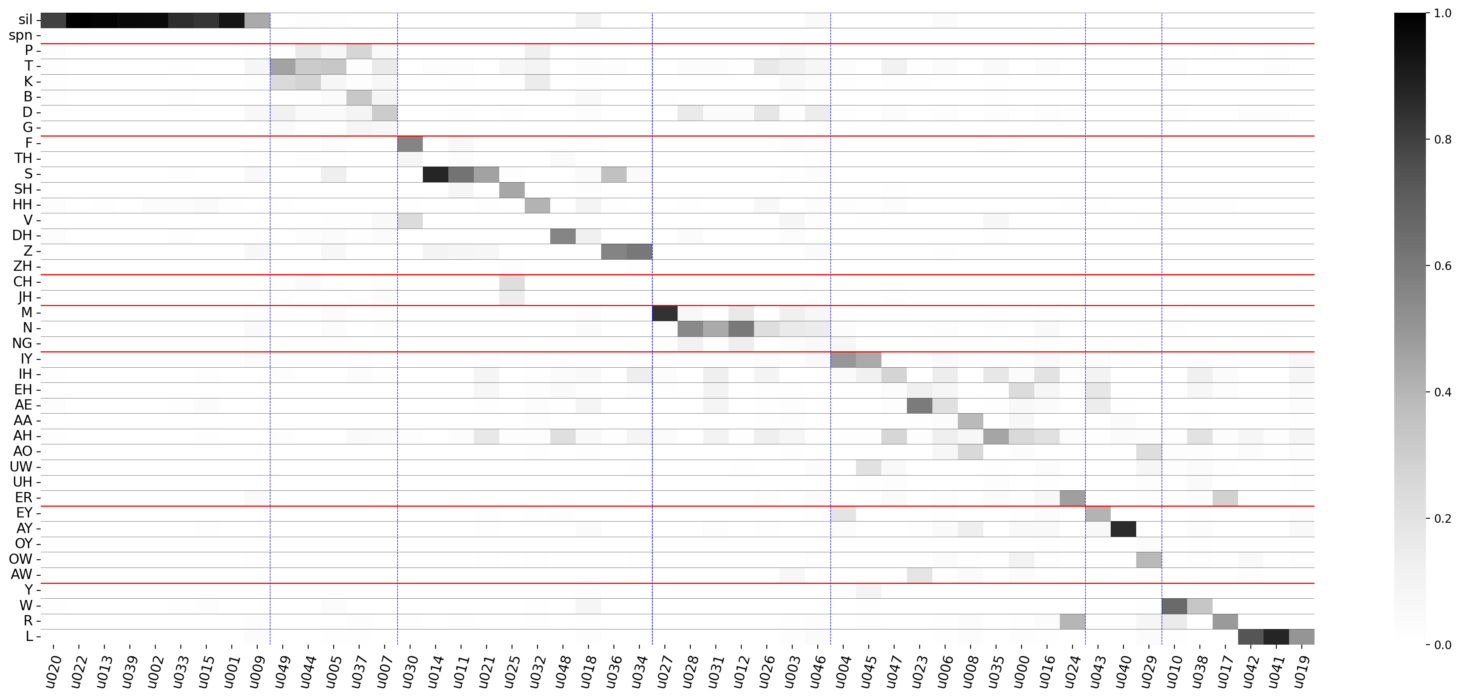
\includegraphics[width=1\linewidth]{feasiblefigs/ch4figs/hub-u050-ap0000-givenunit-byphn.png}
    \caption{hub-u050-ap0000-givenunit-byphn}
    \label{fig:hub-u050-ap0000-givenunit-byphn--detailed}
\end{figure}

\begin{figure}
    \centering
    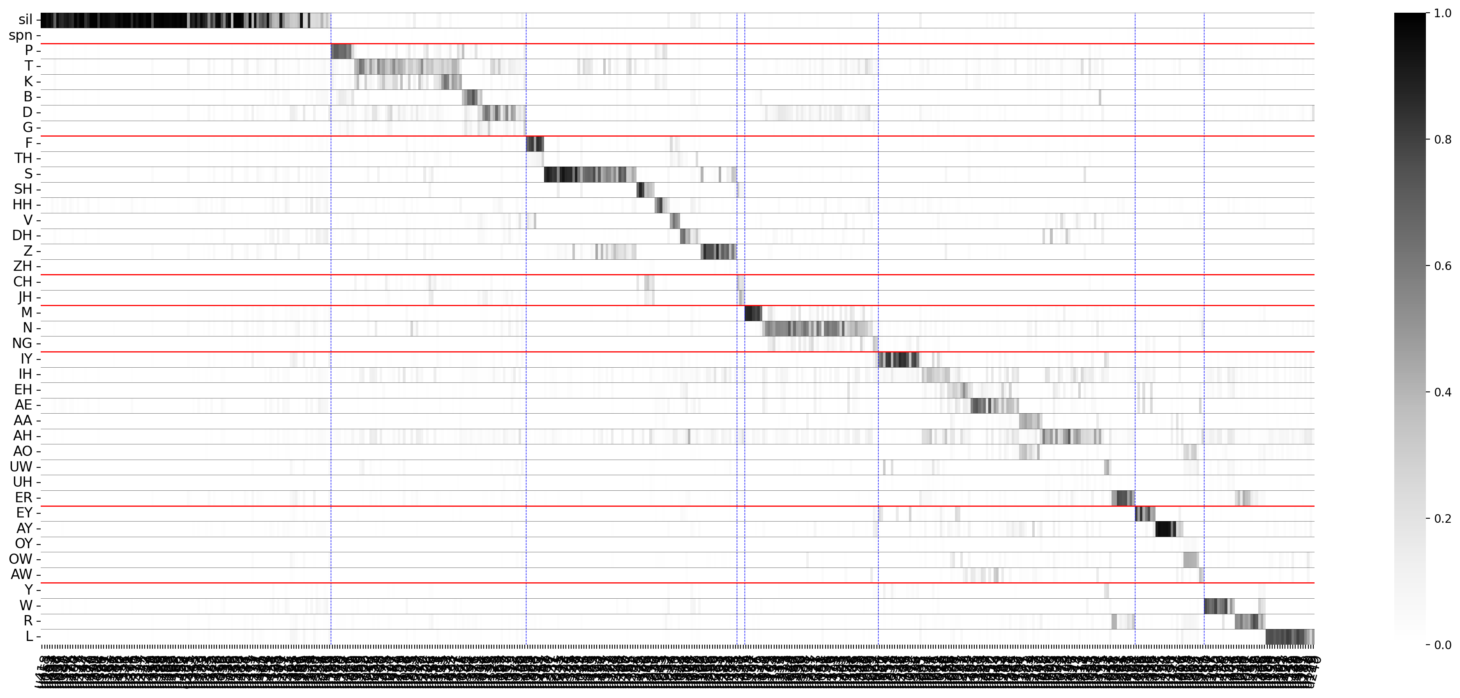
\includegraphics[width=1\linewidth]{feasiblefigs/ch4figs/hub-u050-ap0500-givenunit-byphn.png}
    \caption{hub-u050-ap0500-givenunit-byphn}
    \label{fig:hub-u050-ap0500-givenunit-byphn--detailed}
\end{figure}

\begin{figure}
    \centering
    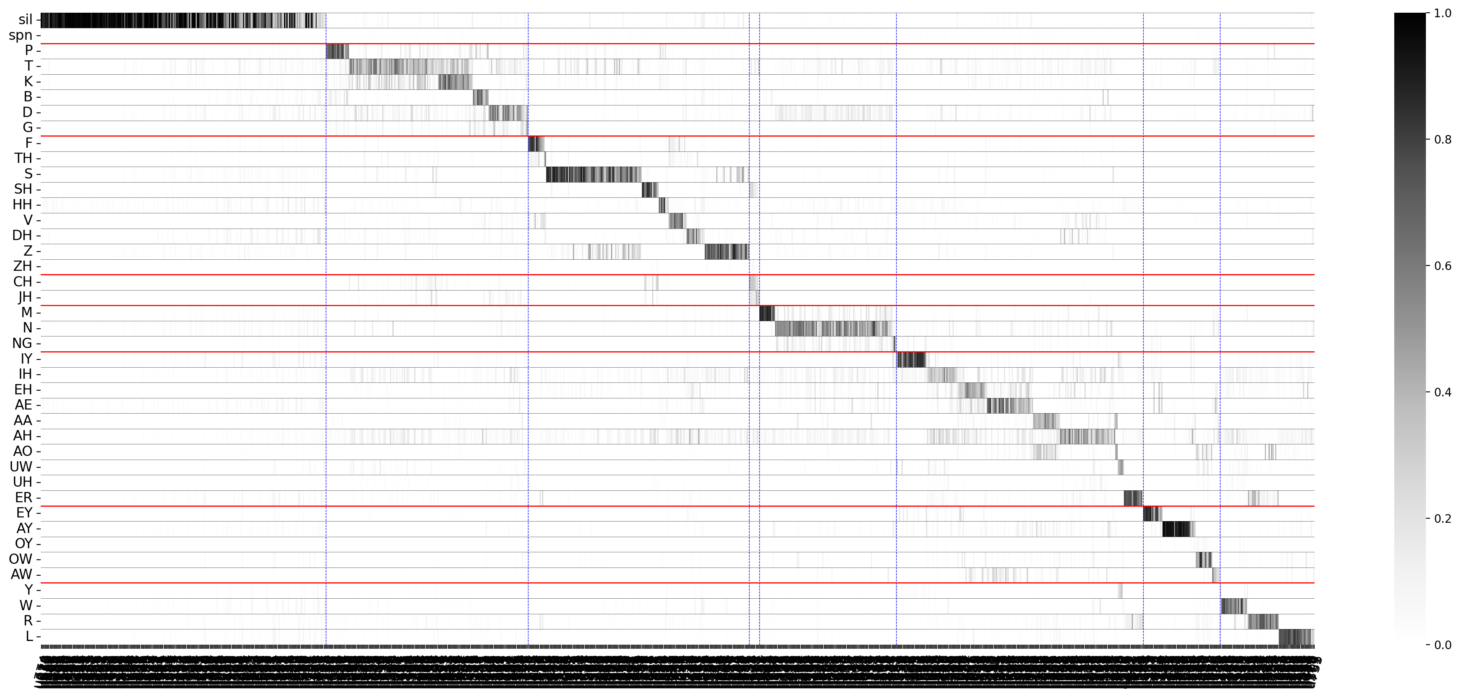
\includegraphics[width=1\linewidth]{feasiblefigs/ch4figs/hub-u050-ap1000-givenunit-byphn.png}
    \caption{hub-u050-ap1000-givenunit-byphn}
    \label{fig:hub-u050-ap1000-givenunit-byphn--detailed}
\end{figure}

\begin{figure}
    \centering
    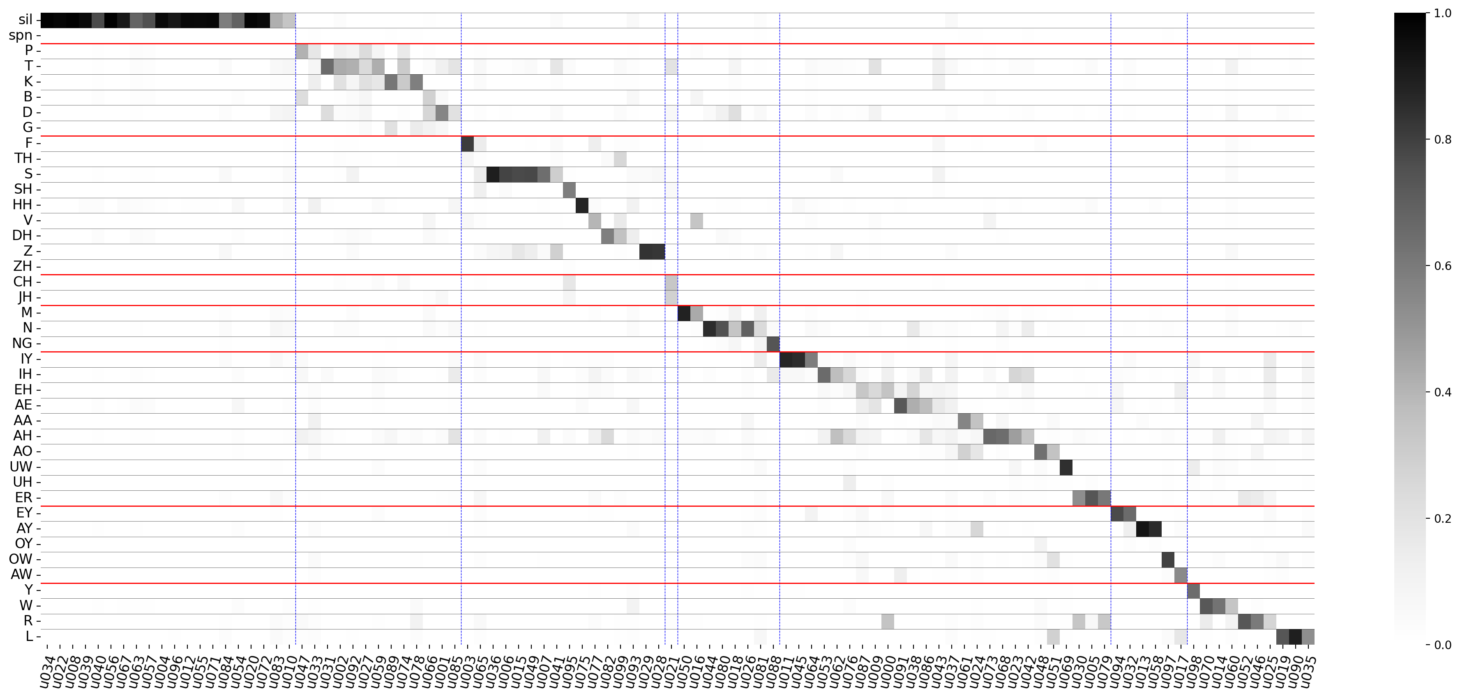
\includegraphics[width=1\linewidth]{feasiblefigs/ch4figs/hub-u100-ap0000-givenunit-byphn.png}
    \caption{hub-u100-ap0000-givenunit-byphn}
    \label{fig:hub-u100-ap0000-givenunit-byphn--detailed}
\end{figure}
\begin{figure}
    \centering
    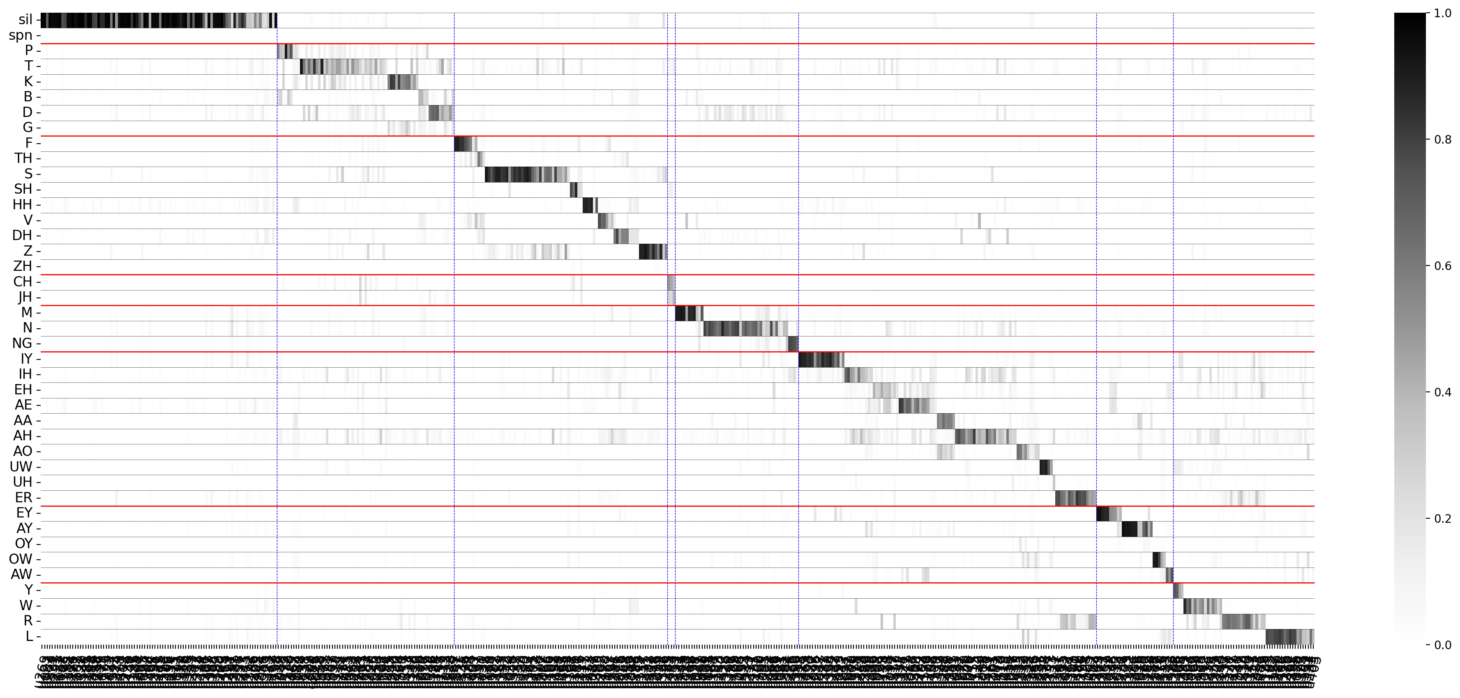
\includegraphics[width=1\linewidth]{feasiblefigs/ch4figs/hub-u100-ap0500-givenunit-byphn.png}
    \caption{hub-u100-ap0500-givenunit-byphn}
    \label{fig:hub-u100-ap0500-givenunit-byphn--detailed}
\end{figure}
\begin{figure}
    \centering
    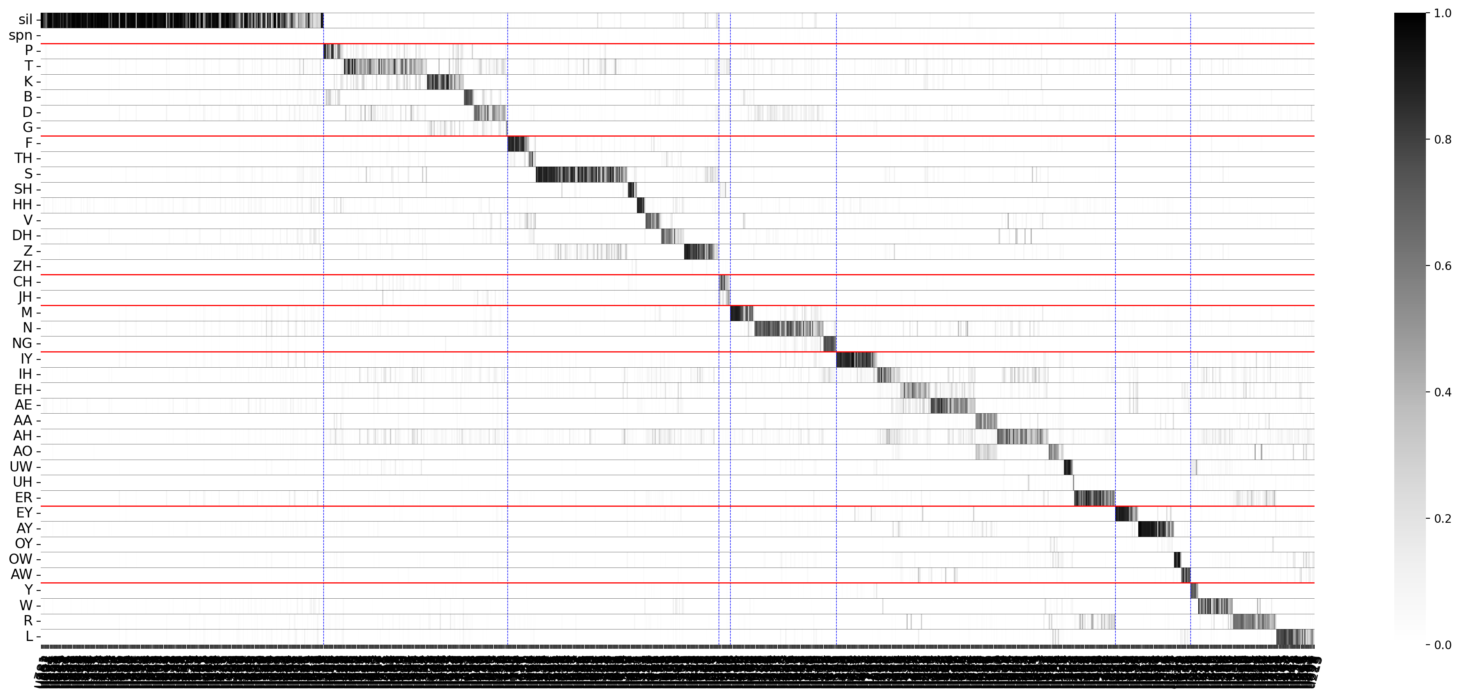
\includegraphics[width=1\linewidth]{feasiblefigs/ch4figs/hub-u100-ap1000-givenunit-byphn.png}
    \caption{hub-u100-ap1000-givenunit-byphn}
    \label{fig:hub-u100-ap1000-givenunit-byphn--detailed}
\end{figure}
}  % heatmaps


\section{本章總結} {   藉由引入分詞演算法我們觀察了用分詞法的效果差異。
}
}

%
